% 课程设计报告：少看少算 —— 从动态特征选择的复现到单趟选块 ViT
% 编译：xelatex report.tex（跑两遍）
\documentclass[11pt,a4paper,UTF8,fontset=none]{ctexart}
\usepackage[a4paper,margin=2.4cm]{geometry}
\setCJKmainfont{Noto Serif CJK SC}[BoldFont={Noto Serif CJK SC Bold}]
\setCJKsansfont{Noto Sans CJK SC}[BoldFont={Noto Sans CJK SC Bold}]
\setCJKmonofont{Noto Sans CJK SC}
\usepackage{amsmath,amssymb}
\usepackage{graphicx}
\usepackage{booktabs}
\usepackage{multirow}
\usepackage[font=small,labelfont=bf,skip=8pt]{caption}
\usepackage{float}
\usepackage{xcolor}
\usepackage{hyperref}
\usepackage{enumitem}
\usepackage{url}
\usepackage{array}
\usepackage{tikz}
\usetikzlibrary{arrows.meta,decorations.pathreplacing}
\setlist{nosep,leftmargin=2em}
\hypersetup{colorlinks=true,linkcolor=black,citecolor=black,urlcolor=blue!60!black}
\setlength{\parskip}{0pt}
\usepackage{indentfirst}
\renewcommand{\arraystretch}{1.15}
\graphicspath{{../results/}}
\newcommand{\term}[1]{\textbf{#1}}
\newcommand{\dense}{整图一次前向}
\newcommand{\fused}{头融合}
\newcommand{\tokdrop}{丢 token}
\newcommand{\onepass}{单趟选块 ViT}

\title{少看少算：从动态特征选择的复现到单趟选块 ViT\\[0.4em]\large 课程设计报告}
\author{}
\date{2026 年 11 月 26 日}

\begin{document}
\maketitle
\thispagestyle{empty}

\begin{abstract}
分类一张图，往往只需要读图中的核心目标；理解一句话，往往只需要读关键的那一段。从特征到答案的信息链真正需要的信息量小于全部特征，于是可以按需取样：用已经读到的特征推断还缺什么，再只读入缺的那部分，用更少的总阅读得到同样的答案。GDFS（Covert 等，ICML 2023）和 DIME（Gadgil 等，ICLR 2024）给出了把“选哪些特征”与“用选中的特征预测”联合训练起来的方法。本报告首先原样复现了它们在 MNIST、CIFAR-10 和 Imagenette 上的图像分类实验，四个实验的曲线都达到或高于论文，预设验收线全部通过。

复现确认了前提：更少的特征确实能保持精度。但两篇工作没有改动网络本身，推理时每读入一块都要把网络从头跑一遍，未读的块置零之后照样经过每一层。实测预算 10 块时，GDFS 的 FLOPs 是\dense 的 14 倍，DIME 是 23 倍：读得更少，算得反而更多。

LLM 的 KV cache 提供了对照：新读入的 token 直接追加到上下文，已缓存的部分不再计算，算量严格等于读入量。我们沿这条思路改了两次 ViT。第一版让未读的块不进入网络，一次前向的算量正比于已读块数，全部块都读入时与原模型逐 logit 相同；它把 FLOPs 从 12 倍压到 0.72 倍，单图延迟仍远高于整图一次前向，因为延迟等于前向次数乘每次前向的固定成本，而串行结构的前向次数是 $k+1$。第二版把 $k$ 次前向合成一次：前 2 层读全图，一次选出 10 块，后 10 层只算选中的块。在 Imagenette 上，预算 10 块时它的准确率 0.915（三种子；串行 DIME 0.892，串行\tokdrop{} 0.852），FLOPs 是\dense 的 0.24 倍，吞吐场景延迟 0.29 倍，单图场景延迟 0.74 倍；全图层取 4 层时准确率 0.951，与串行方法最好的结果持平。代价是放弃了“读完一块再推断下一块”的按需取样。
\end{abstract}

\tableofcontents
\bigskip

%----------------------------------------------------------------------------------
\section{看一部分就够}

\subsection{按需取样}

判断一张照片里是一辆卡车，不需要把路面、天空和墙面都读清楚，读驾驶室和车轮就够了；理解一句话，也常常只需要读其中关键的那一段，其余都是修饰和铺垫。两个例子说的是同一件事：从输入到答案，中间要经过一串特征，真正起作用的只是其中一部分。既然答案只依赖一部分输入，就没有必要把全部输入都读一遍。

\begin{figure}[t]
\centering
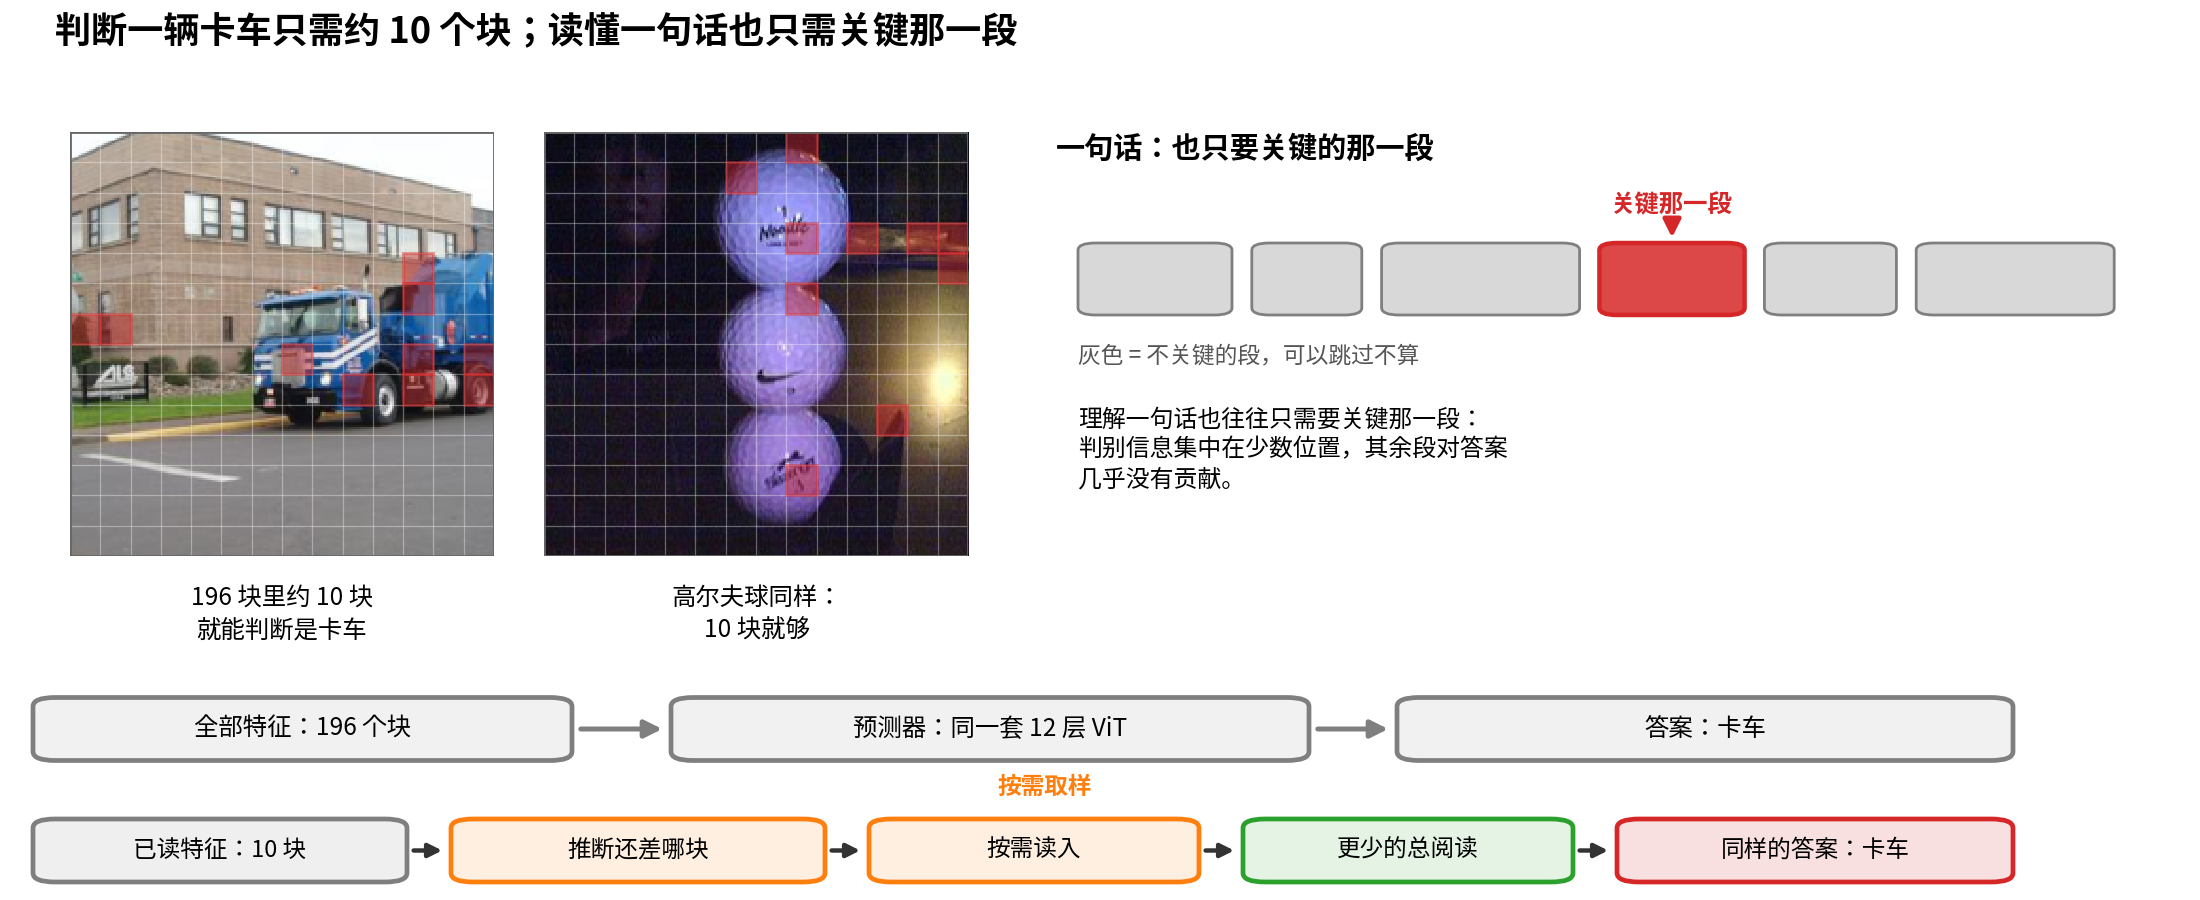
\includegraphics[width=\textwidth]{report_fig01_concept.png}
\caption{只读一部分就够。左、中：模型在预算 10 块时读入的块（红色），足以判断类别；右：一句话里往往只有一段是关键；下：按需取样用更少的总阅读得到同样的答案。}
\label{fig:concept}
\end{figure}

把这件事放到图像分类模型上。模型把一张 $224\times224$ 的图切成 196 个 $16\times16$ 的小块，下面叫\term{块}，英文 patch；每块变成一个向量，称为 token，送进网络得到类别。本文把模型获取一块的特征叫\term{读}这块。如果只有十来块决定类别，就存在一个比“随机少读”更好的策略：先读一部分，根据读到的内容\term{推断还缺哪块}，再按需读入缺的那块，直到足以判断。这就是\term{按需取样}。

它用更少的总阅读得到同样的答案，在读取有成本的场景里本身就是目的；在读取免费、计算有成本的场景里，还有一个自然的期望：读得少，就应该算得少。

\subsection{把直觉变成可训练的方法}

难点在于模型怎么推断“还缺哪块”。两篇被复现的工作给出了同一个思路：训练一个\term{预测器}，它只根据已读的特征预测类别；再训练一个\term{选择器}，它从已读的内容里挑出“对预测最有用的下一块”。两者联合训练，选择器从预测器的损失变化里学到什么叫“有用”。选择是离散的，梯度本来传不过去，两篇工作的区别就在于怎么绕开这一点。

GDFS 用可微松弛绕开这一点：选择器从 Concrete 分布里抽一个块，以温度 $T$ 做 Gumbel-softmax，温度从 2.0 退火到 0.1，梯度经直通估计回到选择器；预测器先用随机掩码预训练，使它在任意子集上都能预测。DIME 则不放松选择，而是训练一个\term{价值网络}，直接回归“再读入某个候选块能让损失下降多少”：
\begin{equation}
\Delta_j = \ell\big(f(x_S), y\big) - \ell\big(f(x_{S \cup \{j\}}), y\big),
\end{equation}
其中 $S$ 是已读集合，$f$ 是预测器，$\ell$ 是损失。推理时每一步价值网络给所有候选块打分，读入分最高的一块。停止准则有三种：预算式（恰好读 $k$ 块）、置信式（预测的最大类概率超过阈值）、惩罚式（预测的改善低于阈值 $\lambda$）。

两篇工作都假设：只要选得准，读得少就能保持精度。这个假设是否成立，不能靠方法描述来判断，只能把实验原样跑一遍。

%----------------------------------------------------------------------------------
\section{复现：少读确实能保持精度}

\subsection{设置}

检验这个假设，先要把两篇工作的实验原样跑通。四个实验沿用作者脚本的数据、划分、模型和训练阶段：GDFS 在 MNIST（像素即特征）和 CIFAR-10（$8\times8$ 个 $4\times4$ 块）上做，DIME 在 MNIST 和 Imagenette（ViT-S/16，$14\times14$ 个 $16\times16$ 块）上做。Imagenette 的训练集按作者方式切出 10\% 做验证，官方 val 文件夹做测试，共 3924 张。

实现是纯 PyTorch 逐行移植，因为作者使用的 Lightning 1.x 与新硬件需要的 torch 版本不兼容；训练与精度评测在 RTX PRO 5000 上以 bf16 运行。延迟另测：训练时 PRO 5000 上同时有多个任务，读数受干扰；为拿到干净数字，所有延迟改在一张空闲的 RTX 5060（8 GB，WSL）上重测，该卡没有其他计算任务。两处硬件不同，延迟只比较同一张卡上的相对倍数，不跨卡比较绝对毫秒；FLOPs 与硬件无关，仍用原测量。与作者设定的偏离列在附录~\ref{app:dev}，都在框架或脚本缺陷层面，不改变语义。表~\ref{tab:setup} 汇总四个实验的设置与训练代价。

\begin{table}[H]
\centering
\caption{四个复现实验的设置与训练代价。}
\label{tab:setup}
\small
\begin{tabular}{lllll}
\toprule
实验 & 数据 & 特征 & 模型 & 训练代价 \\
\midrule
GDFS MNIST & MNIST & 784 个像素 & 两个 MLP & 1.38 GPU 小时 \\
GDFS CIFAR-10 & CIFAR-10 & $8\times8$ 个 $4\times4$ 块 & ResNet 骨干 + 选择头 & 3.35 GPU 小时 \\
DIME MNIST & MNIST & 784 个像素 & 两个 MLP，第一层共享 & 1.40 GPU 小时 \\
DIME Imagenette & Imagenette2-320 & 196 个 $16\times16$ 块 & ViT-S/16（预训练） & 14.2 GPU 小时 \\
\bottomrule
\end{tabular}
\end{table}

\subsection{GDFS}

\begin{table}[H]
\centering
\caption{GDFS 在 MNIST 上的复现：像素预算下的 top-1 准确率。论文数字来自 GDFS Table 3。}
\label{tab:gdfs-mnist}
\small
\begin{tabular}{lcccc}
\toprule
像素预算 & 5 & 10 & 20 & 50 \\
\midrule
复现 & 0.702 & 0.876 & 0.943 & 0.973 \\
论文 & 0.695 & 0.875 & 0.950 & 0.975 \\
差值 & +0.007 & +0.001 & $-$0.007 & $-$0.002 \\
\bottomrule
\end{tabular}
\end{table}

\begin{table}[H]
\centering
\caption{GDFS 在 CIFAR-10 上块预算下的 top-1 准确率，以及三类静态基线。复现与论文读数各占一行；论文数字从 Fig.3 读出（误差约 $\pm0.02$），是 5 次运行的平均。我们的基线每个预算独立训练一次，随机掩码每个预算只抽一组随机块；中心裁剪的预算是 4 / 9 / 16 块，不是 5 / 10 / 15 块。}
\label{tab:gdfs-cifar}
\small
\begin{tabular}{lcccccc}
\toprule
块预算 & 5 & 10 & 15 & 20 & 30 & （1 块） \\
\midrule
GDFS 复现（贪心） & 0.664 & 0.785 & 0.832 & 0.846 & 0.862 & 0.276 \\
GDFS 论文（贪心） & 0.55 & 0.74 & 0.81 & 0.84 & 0.86 & 0.27 \\
\midrule
中心裁剪，复现 & 0.429 & 0.667 & 0.804 & 0.817 & 0.874 & \\
中心裁剪，论文读数 & 0.43 & 0.63 & 0.72 & 0.77 & 0.80 & \\
\midrule
随机掩码，复现（单次抽样） & 0.247 & 0.595 & 0.501 & 0.715 & 0.767 & 0.169 \\
随机掩码，论文读数 & 0.42 & 0.63 & 0.72 & 0.76 & 0.80 & \\
\midrule
CAE，复现 & 0.503 & 0.546 & 0.737 & 0.788 & 0.856 & \\
CAE，论文读数 & 0.50 & 0.72 & 0.78 & 0.82 & 0.84 & \\
\bottomrule
\end{tabular}
\end{table}

先核对 GDFS 在 MNIST 上的结果，它回答的是“复现是否忠实”这个最基本的问题。四个预算点与论文逐点重合，差值都在 0.7 个点以内。在这种量级的差距下，可以认为复现没有引入额外的偏差。

CIFAR-10 上的结论更细。20 块以上与论文重合，5 块和 10 块处复现高出 4--11 个点；论文提到极小预算时贪心选择会略低于基线，这个现象没有复现出来。

更值得注意的是与静态基线的对比。中心裁剪、随机掩码和 CAE 都不依赖已读内容：中心裁剪固定读图像中央，随机掩码每个预算抽一组随机块，CAE 则用可微目标学一组固定的块。动态选择在每一个预算上都高于这三类方案，说明“从已读内容推断下一块”确实比任何固定规则选得好。

\subsection{DIME}

\begin{table}[H]
\centering
\caption{DIME 在 MNIST 上的复现。预算式的论文数字从 Fig.2 读出，惩罚式的论文说法是“约 10 个特征过 90\%”。}
\label{tab:dime-mnist}
\small
\begin{tabular}{llccc}
\toprule
准则 & 参数 & 平均特征数 & 复现 & 论文 \\
\midrule
预算 & $k=5$ & 5 & 0.691 & 约 0.60 \\
预算 & $k=10$ & 10 & 0.874 & 约 0.82 \\
预算 & $k=20$ & 20 & 0.943 & 约 0.92 \\
惩罚 & $\lambda=0.005$ & 12.4 & 0.944 & \\
惩罚 & $\lambda=0.03$ & 9.1 & 0.914 & 约 10 个特征过 0.90 \\
置信 & 0.9 & 10.0 & 0.918 & \\
\bottomrule
\end{tabular}
\end{table}

\begin{table}[H]
\centering
\caption{DIME 在 Imagenette 上的复现（ViT-S/16）。论文数字从 Fig.4 读出（误差约 $\pm0.02$）。}
\label{tab:dime-imagenette}
\small
\begin{tabular}{llccc}
\toprule
准则 & 参数 & 平均块数 & 复现 & 论文 ViT \\
\midrule
预算 & $k=2$ & 2 & 0.614 & 0.37 \\
预算 & $k=4$ & 4 & 0.743 & 0.50 \\
预算 & $k=10$ & 10 & 0.892 & 0.75 \\
预算 & $k=15$ & 15 & 0.926 & 0.84 \\
预算 & $k=30$ & 30 & 0.961 & \\
惩罚 & $\lambda=0.024$ & 9.8 & 0.954 & 10 块 0.94 \\
惩罚 & $\lambda=0.018$ & 11.1 & 0.962 & 12 块 0.96 \\
惩罚 & $\lambda=0.01$ & 13.8 & 0.975 & 15 块 0.97 \\
置信 & 0.9 & 7.8 & 0.919 & \\
\bottomrule
\end{tabular}
\end{table}

\begin{figure}[t]
\centering
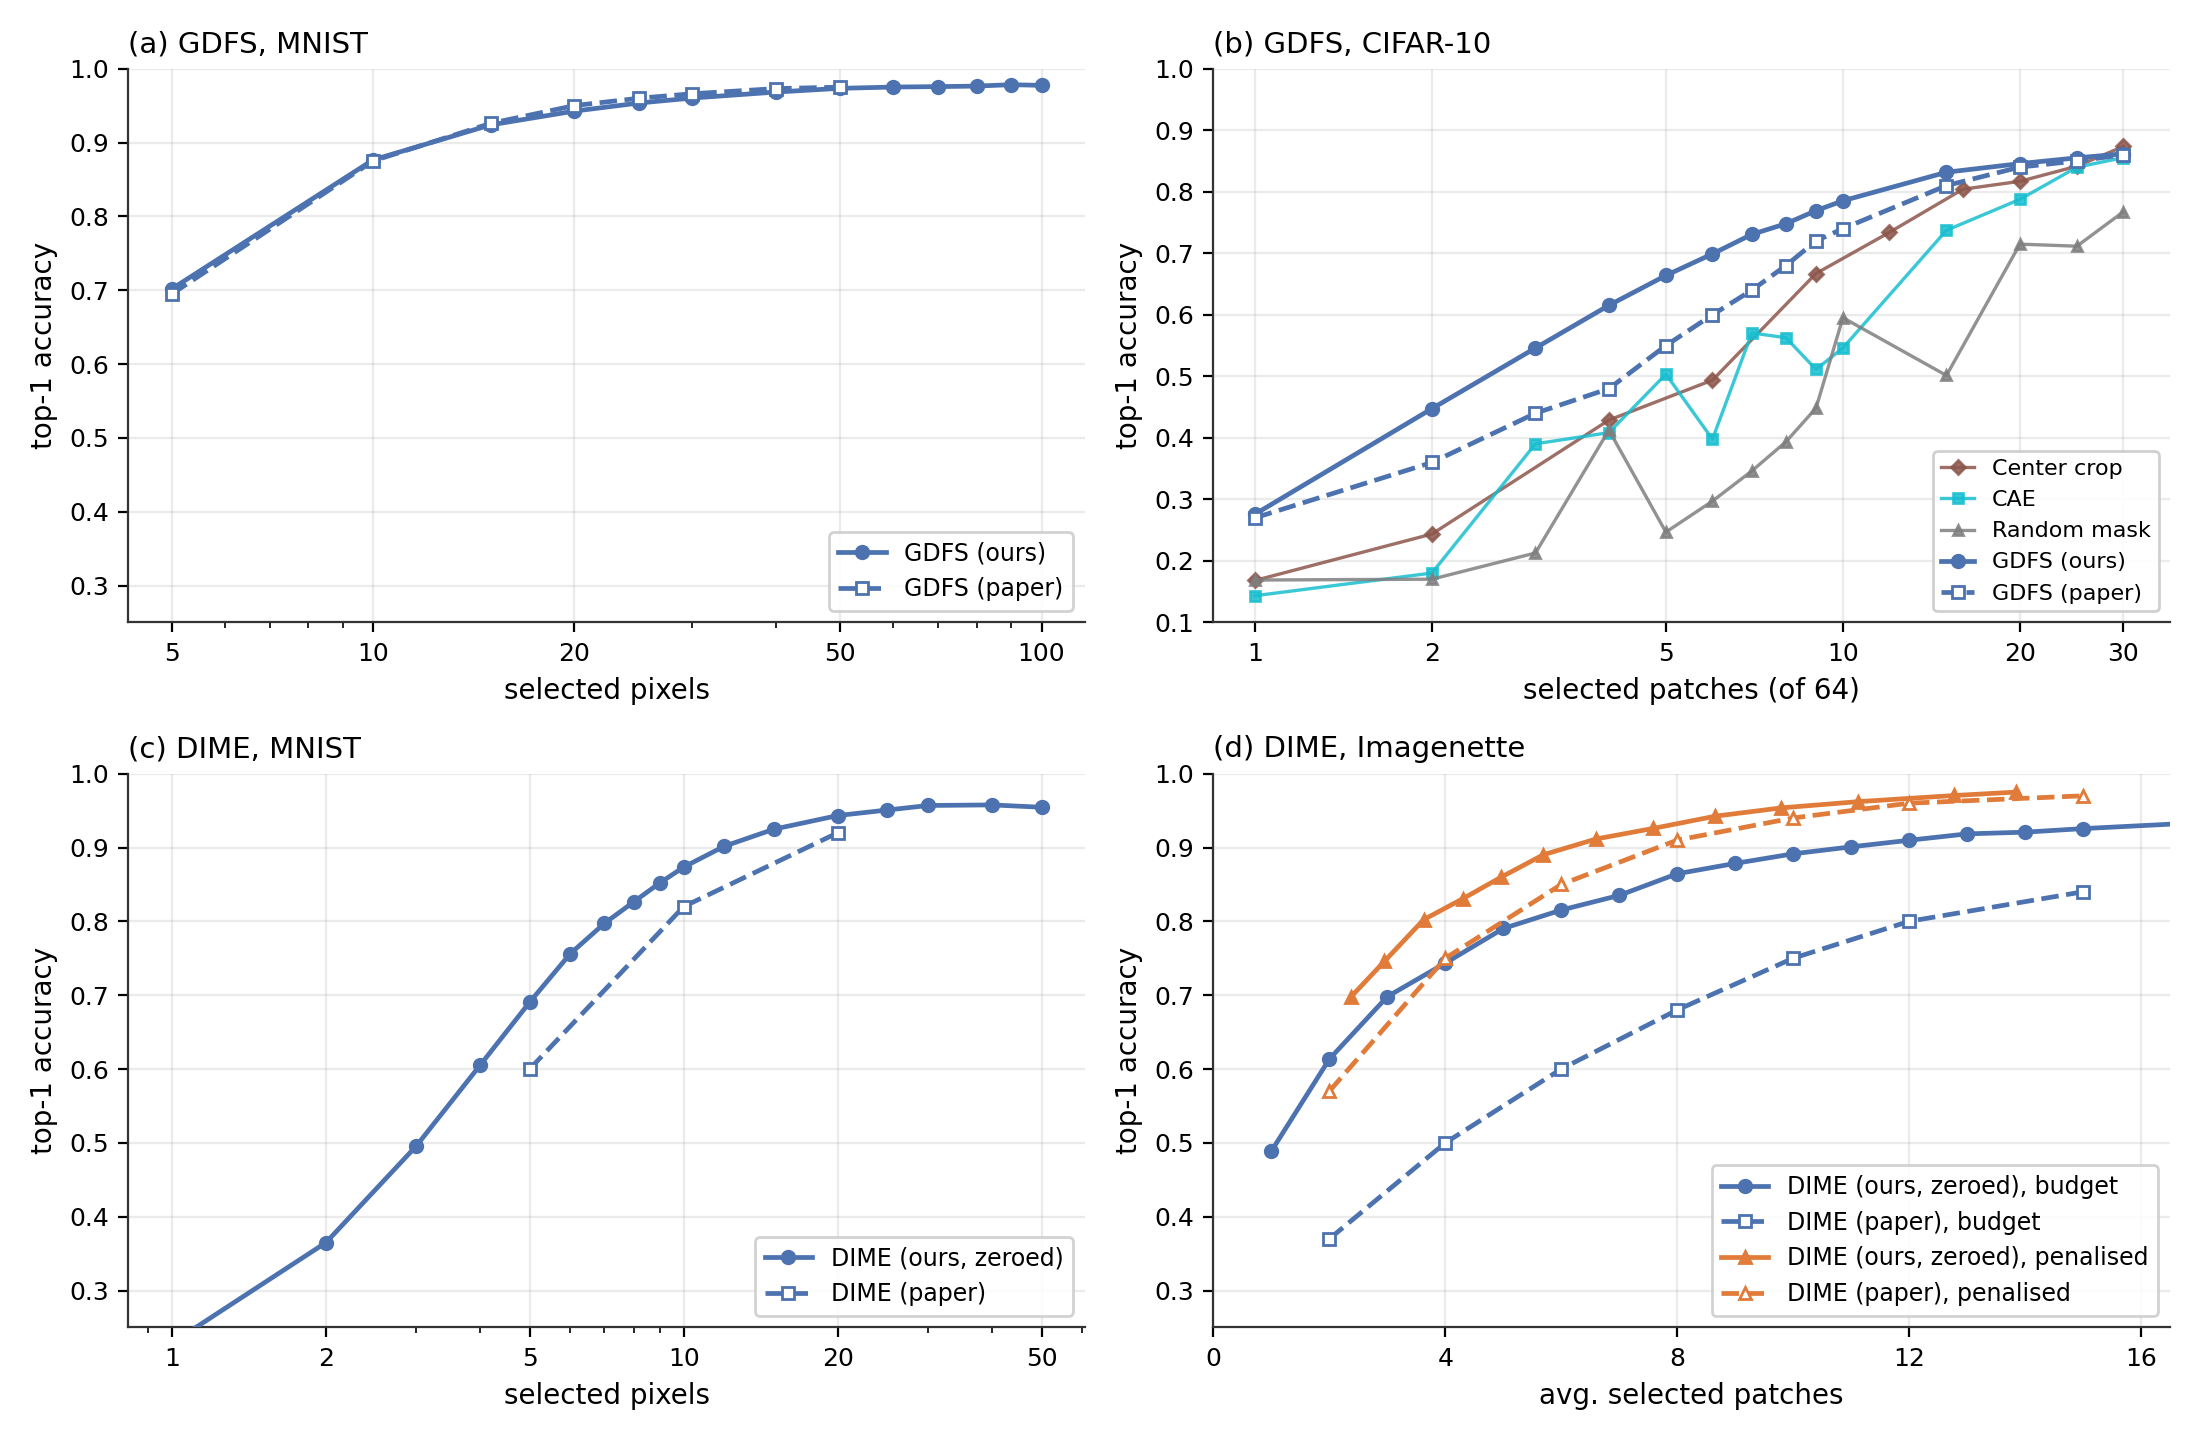
\includegraphics[width=\textwidth]{report_fig05_reproduction.png}
\caption{四个复现实验：复现（实线，实心点）与论文读数（虚线，空心点）。(a) GDFS MNIST；(b) GDFS CIFAR-10，含我们复现的三类静态基线（每条一次独立训练，曲线因此不单调）；(c) DIME MNIST 预算式；(d) DIME Imagenette 预算式与惩罚式。}
\label{fig:reproduction}
\end{figure}

DIME 的选择器换成价值网络后，复现的形态不同，需要分别讨论两个数据集。MNIST 上预算式曲线比论文读数高 2--9 个点，惩罚式在 9--12 个特征处都过 0.91。复现不仅没有掉点，反而普遍略高，说明前提在像素特征上同样成立。

Imagenette 上，惩罚式曲线与论文重合，预算式曲线在 10--15 块处比论文高 9--14 个点，小预算处差距更大，我们的预算曲线反而更接近论文的惩罚曲线。“惩罚式优于预算式”这个结论复现出来了，但差距只有 6 个点，论文约 19 个点。

整图（196 块）的测试准确率是 0.994，这是后面所有“少读”方法要逼近的上限。

\subsection{前提成立}

四个实验合起来说明：在 10 块左右，按需取样能拿到整图精度的大部分，而且高于任何不依赖已读内容的静态方案。前提成立，“少读”是可行的。这个结论只关于精度，不关于代价；代价要等把推理过程拆开之后才能算清。

复现过程中有一个工程教训值得记一笔，它说明读数必须回到推理代码里核对。DIME 的预算式推理在“所有样本都已停止”的那一轮漏写了最终预测，训练结束时的自动评测因此给出 0.114；修复后用最终权重重评，上面的表是修复后的数字。问题出在推理函数，训练本身不受影响。

%----------------------------------------------------------------------------------
\section{悖论：读得更少，算得更多}

\subsection{数一数前向次数}

两篇工作只训练了选择器和预测器，推理时网络怎么跑没有动。本文把网络从头到尾跑一遍叫\term{一次前向}。GDFS 每读入一块跑一次选择器网络，读完后跑一次预测器，预算 $k$ 需要 $k+1$ 次前向。DIME 每一步让价值网络和预测器各跑一次骨干，最后再跑一次预测，预算 $k$ 需要 $2(k+1)+1$ 次，$k=10$ 时是 23 次。

串行不是实现偷懒，而是这种设计的本质。每一步的选择依赖上一步读入之后网络读到了什么，所以必须等上一次前向结束；按需取样的“推断还缺哪块”就藏在这一前一后里。于是问题变成：这些前向里有多少计算是必要的？

\begin{figure}[t]
\centering
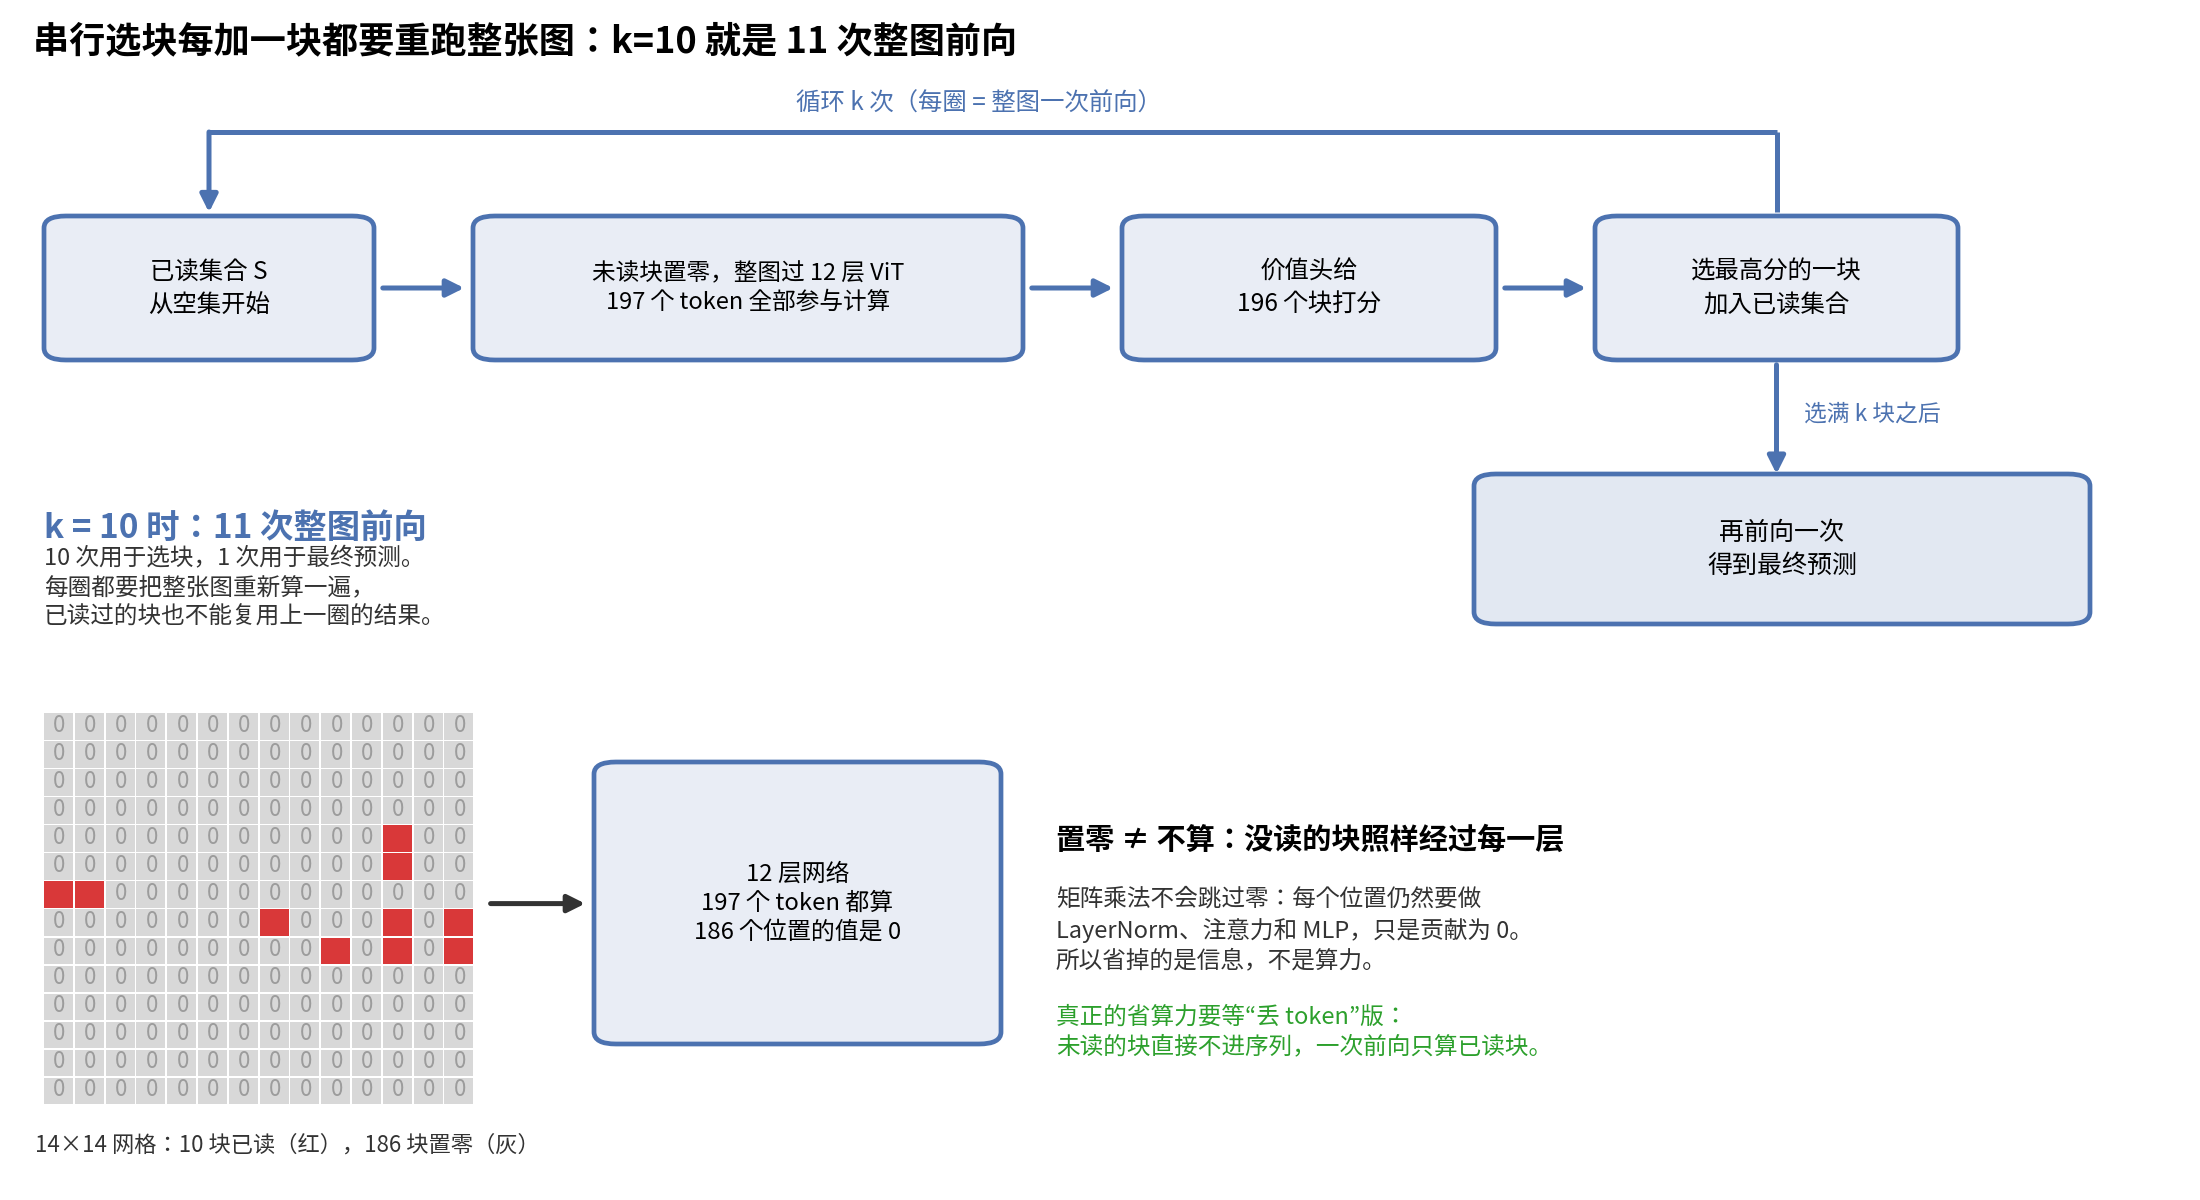
\includegraphics[width=\textwidth]{report_fig02_sequential.png}
\caption{串行按需取样怎么工作、代价在哪。上：每读入一块都要把网络从头跑一遍，$k=10$ 时共 11 次前向；下：未读的块被置零后照样经过每一层，置零不等于不算。}
\label{fig:sequential}
\end{figure}

图~\ref{fig:sequential} 里还有第二层浪费。为了告诉网络“哪些块已经读了”，CIFAR 和 ViT 版本都把未读的块\term{置零}，整张图照样进入网络。置零不等于不算：值为零的块同样参与每一层卷积和注意力，消耗的算力与有值的块完全一样。

直觉上，没读的特征根本不应该被算。但这个直觉值多少算力，不能靠想，得把开销实际量出来。

\subsection{算力开销}

先算算力。本文用 FLOPs（浮点运算次数，按 $2\times\mathrm{MACs}$ 计）度量计算量，参照是\dense：同一骨干读入全部特征跑一遍。表~\ref{tab:flops} 给出预算 10 块时推理的总 FLOPs 与参照的比值，用 torch 的 FlopCounterMode 在同一张卡上实测。

\begin{table}[H]
\centering
\caption{预算 10 块时的 FLOPs 对比，相对\dense。}
\label{tab:flops}
\small
\begin{tabular}{llll}
\toprule
模型 & \dense & $k=10$：作者代码 & $k=10$：\fused \\
\midrule
GDFS MNIST（MLP） & 2 MFLOPs & 14.7$\times$ & 不适用（两个独立网络） \\
GDFS CIFAR-10（ResNet） & 0.51 GFLOPs & 14.1$\times$ & 不适用 \\
DIME MNIST（MLP） & 2 MFLOPs & 27.1$\times$ & 27.1$\times$（两个网络不能共享） \\
DIME Imagenette（ViT-S/16） & 9.2 GFLOPs & 23$\times$ & 12$\times$ \\
\bottomrule
\end{tabular}
\end{table}

读入的像素只有二十分之一，算力却是 14 到 23 倍。差距来自结构：读入量按块计，计算量按整图计，两者脱钩。DIME 的两个头共用同一个骨干，把两次前向合成一次（下文叫\term{\fused}）可以不减任何计算就省一半，输出逐元素相同；这是不改模型就能拿到的 2 倍，之后仍剩 12 倍。

\begin{figure}[t]
\centering
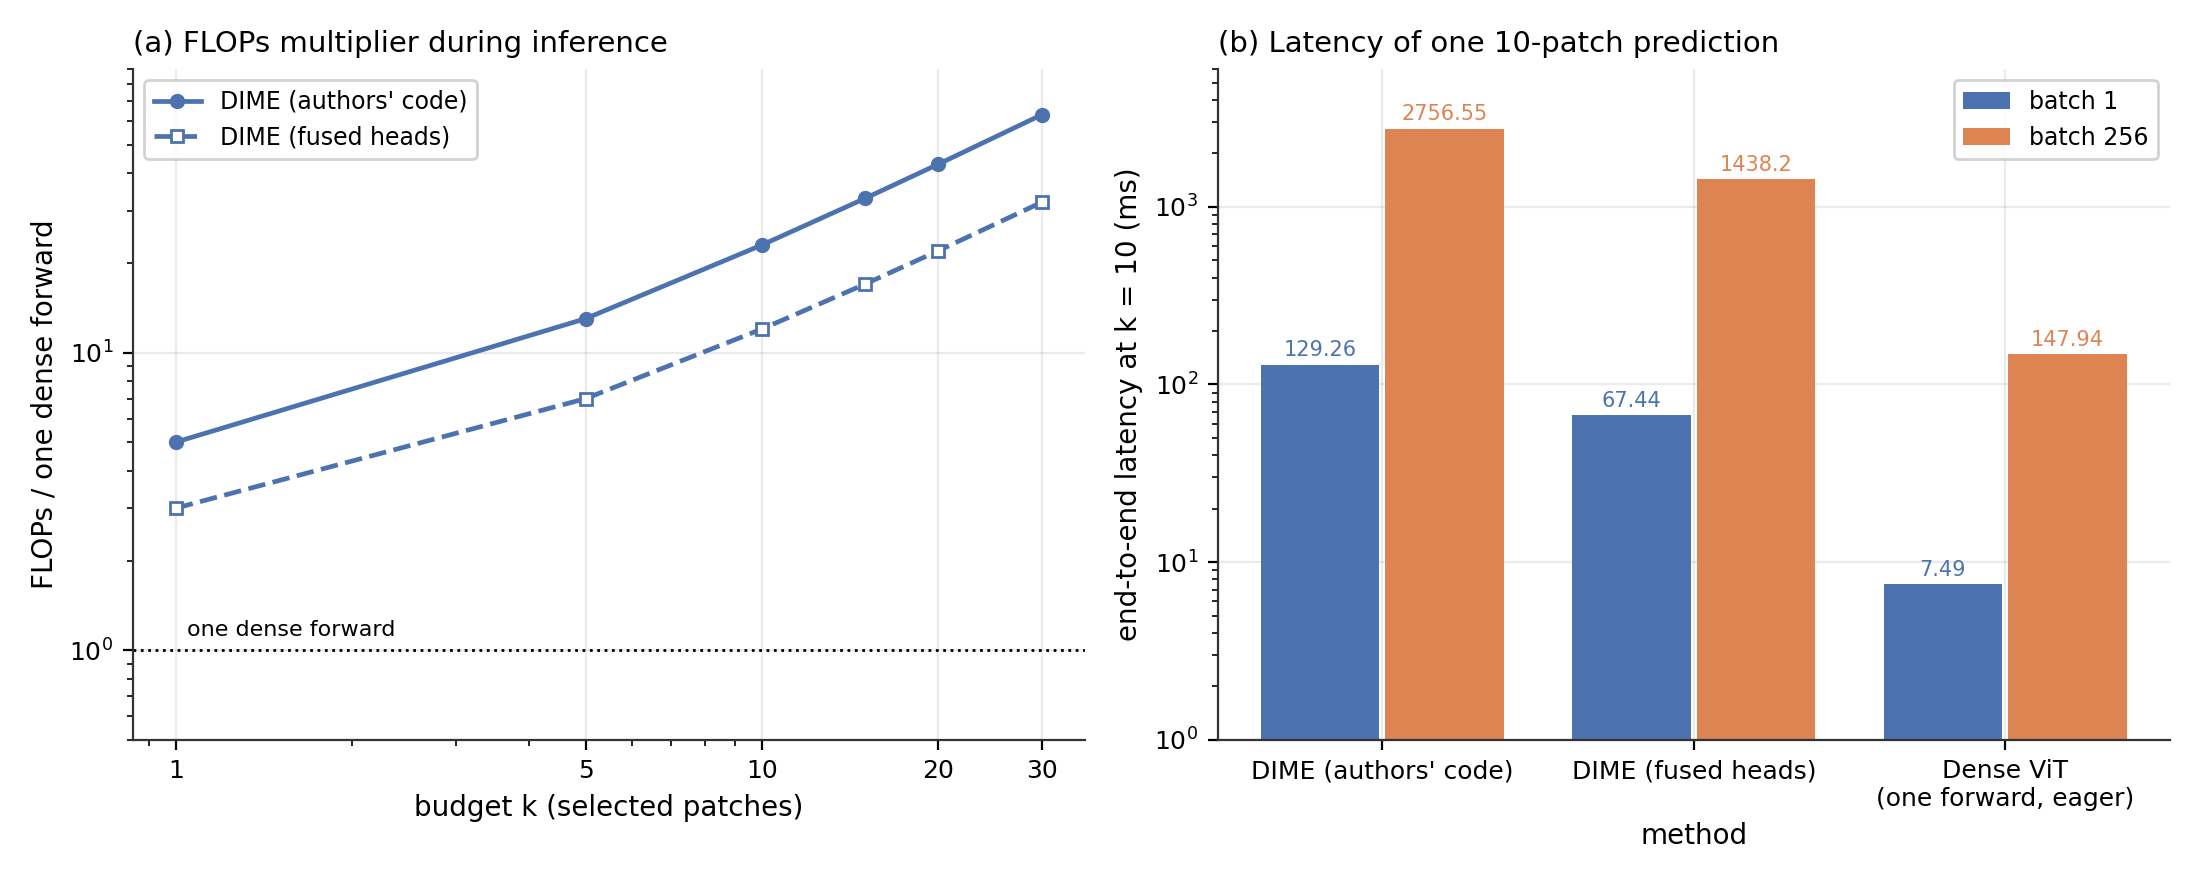
\includegraphics[width=\textwidth]{report_fig07_paradox.png}
\caption{按作者代码的推理方式，预算 10 块的代价比\dense 高一个数量级（Imagenette，DIME）。左：FLOPs 相对\dense 的倍数随预算增长，两个头合成一次前向（\fused）只能减半；右：预算 10 块时的全程延迟，batch 1 与 batch 256，参照是一次 eager 的整图前向。}
\label{fig:ledger}
\end{figure}

\subsection{置零的块能不能跳过}

对 CNN 有一个直接的设想：保留置零的做法，用块稀疏卷积核只计算感受野碰到已读块的输出点。这样未读块虽然还在张量里，却不参与有效计算。这个设想能省多少，取决于已读块在空间上有多集中。我们在 CIFAR-10 测试集的真实选择上逐层统计了理想情况（零开销的理想核）能省的比例，见表~\ref{tab:sparse}。

\begin{table}[H]
\centering
\caption{稀疏卷积在 GDFS CIFAR-10 上的上界（2000 张测试图的真实选择）：理想块稀疏卷积核能省的 FLOPs 比例。}
\label{tab:sparse}
\small
\begin{tabular}{lcccc}
\toprule
已读块数 $k$ & 1 & 5 & 10 & 20 \\
\midrule
选择器前向可省 & 27.9\% & 13.6\% & 6.7\% & 1.2\% \\
预测器前向可省 & 55.7\% & 27.1\% & 13.4\% & 2.3\% \\
GDFS 推理整体可省 & 37.2\% & 14.8\% & 7.0\% & 1.2\% \\
\bottomrule
\end{tabular}
\end{table}

\begin{figure}[t]
\centering
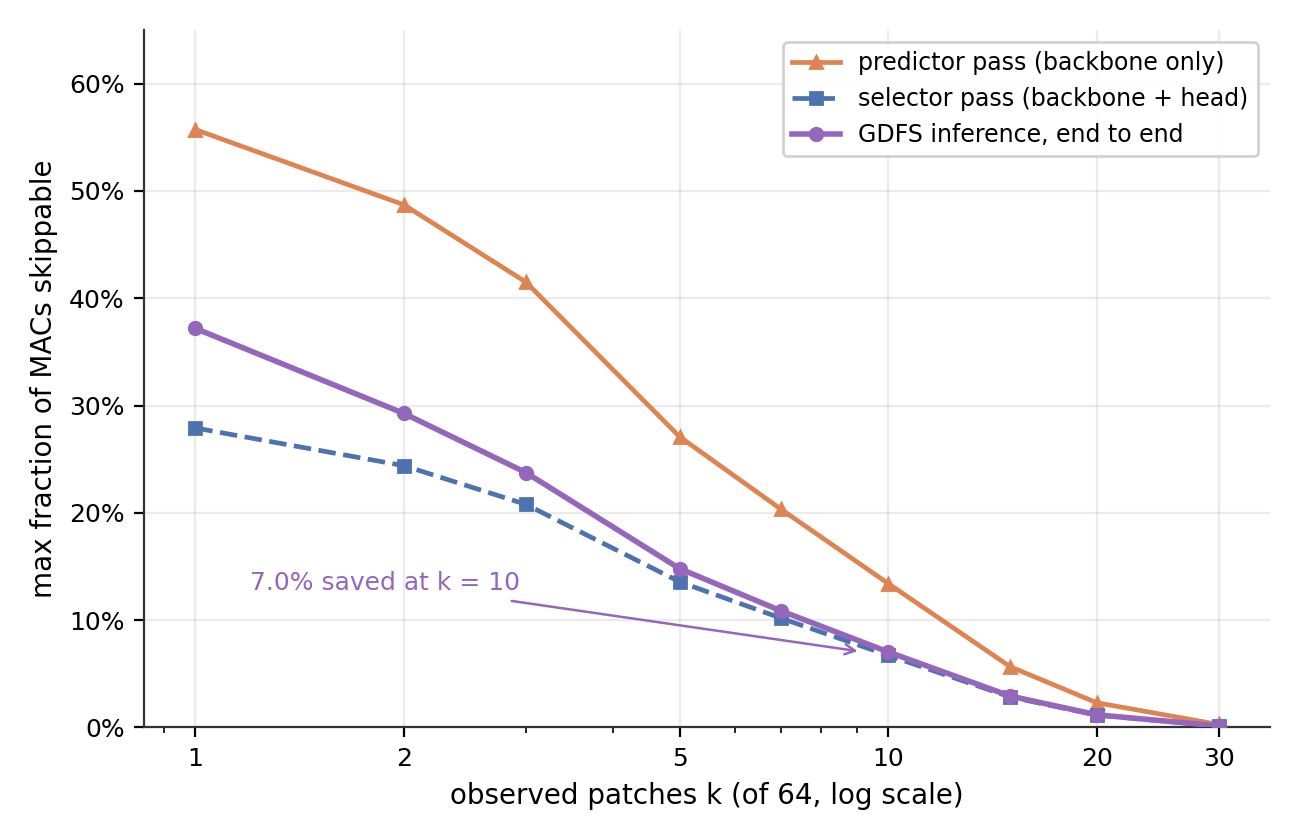
\includegraphics[width=0.7\textwidth]{report_fig08_sparse_bound.png}
\caption{稀疏卷积的可省比例随已读块数迅速下降：预算 10 块时最多省 7\%。}
\label{fig:sparse}
\end{figure}

上界小到几乎没有意义：$4\times4$ 的块在 $32\times32$ 图上太小，到第二层感受野就盖满整图，几乎没有输出点能跳过。稀疏卷积在 CNN 上抵不过 $k+1$ 倍的重跑，所以不在 CNN 上实现稀疏卷积核。真实选择比随机选择聚集一些（随机选 10 块只省 1.8\%），但结论不变。

对 ViT 事情不同。ViT 的每一块就是一个独立的 token，未读的块可以不进入 token 序列，而不是置零后照样算。这指向一个更彻底的做法：让算量真的等于读入量。

%----------------------------------------------------------------------------------
\section{向 LLM 的 KV cache 学：只算读到的}

\subsection{KV cache 做对了什么}

大语言模型逐 token 生成时用 KV cache：已经生成的 token 在每一层的 K、V 缓存起来，新 token 只计算自己那一列，再去读缓存。它做到了两件事：\term{没读到的不算}，\term{算过的不重算}。算量严格等于读入量。

\begin{figure}[t]
\centering
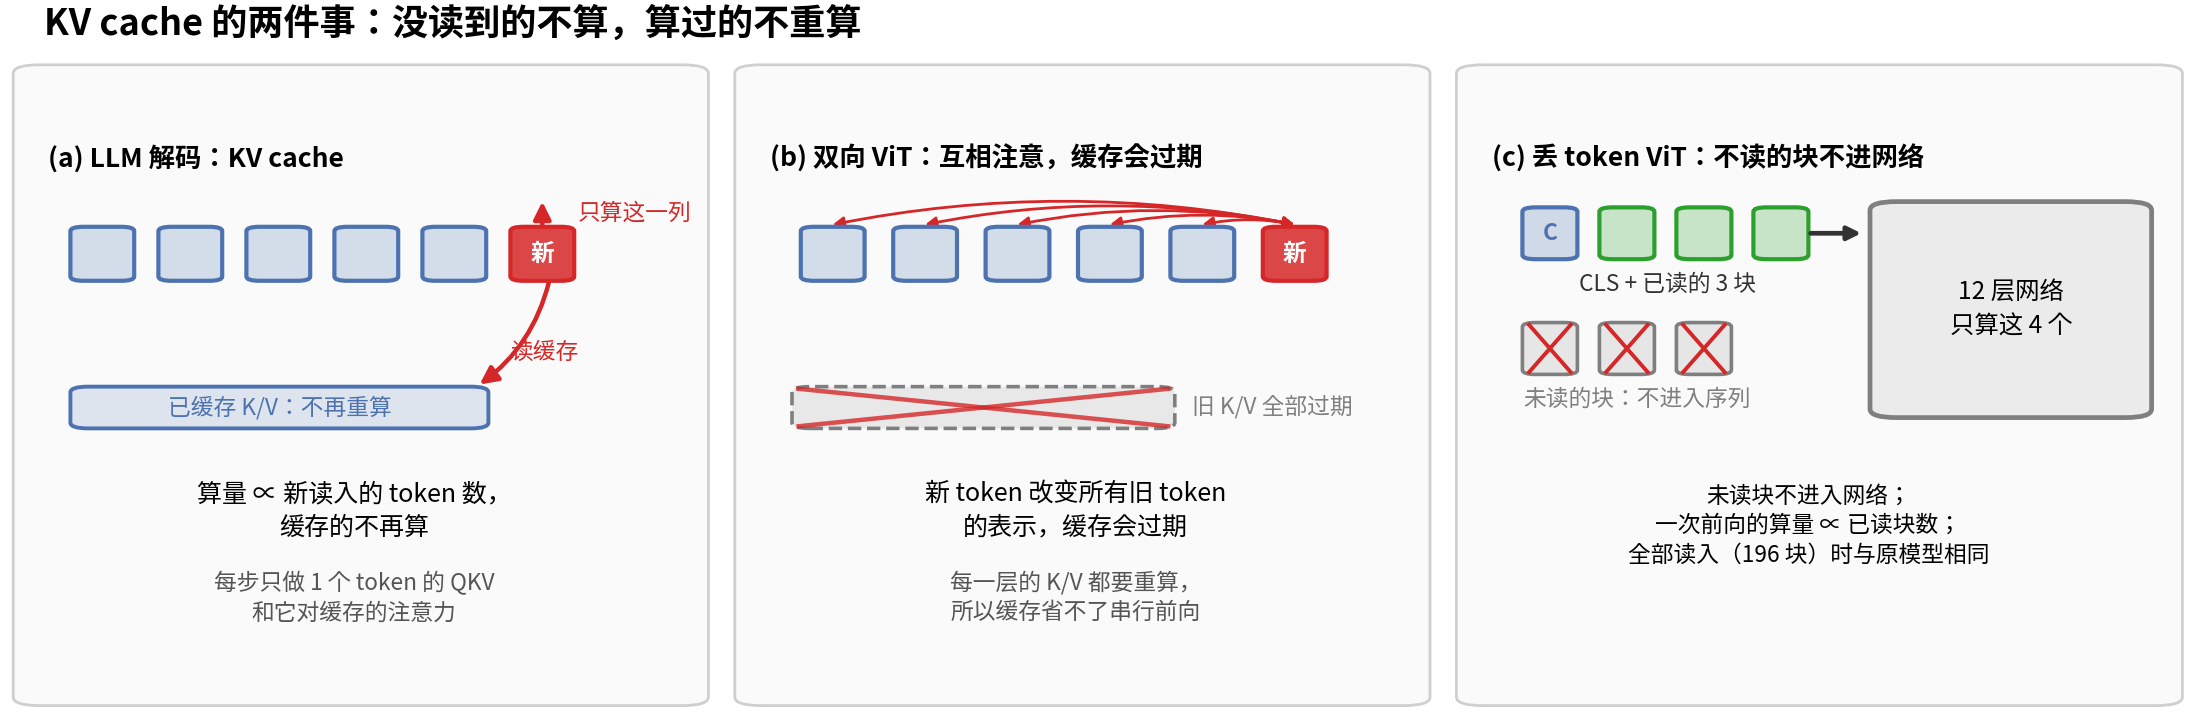
\includegraphics[width=\textwidth]{report_fig03_kvcache.png}
\caption{(a) LLM 的 KV cache：新 token 只算自己并读取缓存，算量正比于新读入的 token 数。(b) 双向 ViT：每个 token 与所有 token 互相注意，加入新 token 会改变所有旧 token 的表示，缓存会过期。(c) 丢 token ViT：未读的块不进入网络，一次前向的算量正比于已读块数；全部读入时与原模型相同。}
\label{fig:kvcache}
\end{figure}

ViT 不能直接套用，因为它是双向注意力：每个 token 与所有 token 互相注意，加入一个新 token 会改变所有旧 token 在每一层的表示，缓存下来的 K、V 立刻过期。LLM 能缓存，是因为因果掩码保证了旧 token 永远看不到新 token。所以两件事要分开做：“没读到的不算”可以在 ViT 上做到；“算过的不重算”在双向结构里做不到精确。

\subsection{第一版改型：丢 token ViT}

\begin{figure}[H]
\centering
\begin{tikzpicture}[
  font=\small,
  >=Latex,
  box/.style={draw, rounded corners=2pt, minimum height=6mm, minimum width=7mm, inner sep=2pt, align=center},
  tok/.style={box, fill=blue!15, draw=blue!55!black},
  cls/.style={box, fill=orange!15, draw=orange!60!black},
  vit/.style={draw, rounded corners=3pt, fill=black!4, minimum width=2.8cm, minimum height=1.8cm, align=center},
  arr/.style={->, thick, draw=black!70},
  lab/.style={font=\scriptsize, text=black!75},
]
\node[anchor=south west, font=\small\bfseries] at (-0.05,0.15) {(a) 读入的块};
\foreach \i in {0,...,13} {
  \foreach \j in {0,...,13} {
    \fill[black!8] (0.18*\i, -0.25-0.18*\j) rectangle ++(0.175,-0.175);
  }
}
\foreach \i/\j in {5/3,6/3,7/3,6/4,7/4,8/4,6/5,7/5,8/5,7/6} {
  \fill[blue!35] (0.18*\i, -0.25-0.18*\j) rectangle ++(0.175,-0.175);
}
\draw[black!25, step=0.18] (0,-0.25) grid (2.52,-2.77);
\fill[blue!35] (0,-3.02) rectangle ++(0.16,-0.16);
\node[lab, anchor=west] at (0.22,-3.10) {已读};
\fill[black!8] (0.85,-3.02) rectangle ++(0.16,-0.16);
\node[lab, anchor=west] at (1.07,-3.10) {未读};

\draw[arr] (2.72,-1.45) -- (3.10,-1.45);

\node[anchor=south west, font=\small\bfseries] at (3.15,0.15) {(b) 构造 token 序列};
\node[cls] (cl) at (3.55,-0.65) {[CLS]};
\node[tok] (t1) at (4.45,-0.65) {$t_{i_1}$};
\node[tok] (t2) at (5.25,-0.65) {$t_{i_2}$};
\node at (5.85,-0.65) {$\cdots$};
\node[tok] (tk) at (6.55,-0.65) {$t_{i_k}$};
\node[lab] at (4.45,-1.04) {$p_{i_1}$};
\node[lab] at (5.25,-1.04) {$p_{i_2}$};
\node[lab] at (6.55,-1.04) {$p_{i_k}$};
\draw[decorate,decoration={brace,amplitude=4pt,mirror},thick] (3.12,-1.15) -- (6.95,-1.15) node[midway,below=5pt,lab] {长度 $1+|S|$};
\node[lab, anchor=north] at (5.0,-1.62) {位置编码按原图位置取，不重新编号};

\draw[arr] (7.05,-0.65) -- (7.45,-0.65);

\node[anchor=south west, font=\small\bfseries] at (7.3,0.15) {(c) 一次前向};
\node[vit] (v) at (8.75,-0.75) {12 层 ViT\\[1pt] 自注意力 + MLP\\[1pt] 键 padding 掩码};
\draw[arr] (10.15,-0.35) -- (10.35,-0.35);
\draw[arr] (10.15,-1.15) -- (10.35,-1.15);
\node[anchor=west, font=\footnotesize, text=black!80] at (10.42,-0.35) {CLS $\to$ 分类头 $\to \hat y$};
\node[anchor=west, font=\footnotesize, text=black!80] at (10.42,-1.15) {196 个位置查询 $\to$ 价值头 $\to s_j$};

\node[anchor=west, font=\small\bfseries] at (0,-3.65) {(d) 算量对比};
\node[anchor=west, lab] at (0,-4.02) {置零};
\draw[fill=black!10, draw=black!25] (0.78,-4.22) rectangle (7.0,-3.92);
\node[anchor=west, lab] at (0.9,-4.07) {197 个 token 全部进入网络};
\node[anchor=west, lab] at (0,-4.55) {删 token};
\draw[fill=blue!20, draw=blue!50] (1.08,-4.75) rectangle (3.7,-4.45);
\node[anchor=west, lab] at (3.85,-4.60) {只进入 $1+|S|$ 个};
\end{tikzpicture}
\caption{\tokdrop{} 的原理与一次前向。(a) 蓝色为已读块，灰色为未读块；(b) 序列只由 CLS 和已读 token 组成，位置编码按原图位置取；(c) 12 层 ViT 只处理这些 token，CLS 进分类头，196 个位置查询经价值头给候选块打分；(d) 与置零版相比，进入网络的 token 数从全部 197 个降到 $1+|S|$ 个。}
\label{fig:tokdrop-arch}
\end{figure}

\term{\tokdrop}对 ViT 的改法是把“置零”改成“删除”。图~\ref{fig:tokdrop-arch} 给出一次前向的完整路径：给定已读集合 $S$，序列只保留 CLS 和 $S$ 中每块对应的 token，长度是 $1+|S|$；未读块不进入序列，也不参与任何一层的注意力。

具体实现上，patch embedding 把卷积权重视为线性层，按已读位置取出 token，未读位置不进入后续张量；位置编码按块在原图中的位置取，不因为删除而重新编号；批内序列长短不一，统一 padding 到批内最长，注意力用 key padding mask 屏蔽 padding；预测头仍是 CLS 上的线性层。

价值头需要单独改。它原来读每个候选位置的 token，候选位置现在没有 token，于是改成 196 个按位置学习的查询向量，用位置编码初始化，对已读 token 和 CLS 做交叉注意力，输出每个候选块的分数；选择时把已读位置的分数屏蔽掉，在未读块里取最高的一个。

它有一个重要的性质：当 196 块全部读入时，它与原模型逐 logit 相同（单元测试验证到 $10^{-3}$）。也就是说它没有放弃原模型的能力，只是在未读的块上不花算力。一次前向的算量正比于已读块数，这是 KV cache 的第一件事。

函数变了：空 token 不再参与注意力，所以要用这个前向重新训练。训练沿用同一协议，80 轮，11.3 GPU 小时。测试集准确率见表~\ref{tab:tokdrop}。

\begin{table}[H]
\centering
\caption{DIME Imagenette 预算式下，置零的稠密 ViT 与\tokdrop{} ViT 的测试准确率（同一训练协议，只有前向方式不同）。}
\label{tab:tokdrop}
\small
\begin{tabular}{lcccccc}
\toprule
块数 & 1 & 4 & 10 & 15 & 20 & 30 \\
\midrule
置零（稠密 ViT） & 0.489 & 0.743 & 0.892 & 0.926 & 0.946 & 0.961 \\
\tokdrop{} & 0.354 & 0.748 & 0.852 & 0.891 & 0.908 & 0.941 \\
差值 & $-$0.135 & +0.005 & $-$0.040 & $-$0.034 & $-$0.038 & $-$0.020 \\
\bottomrule
\end{tabular}
\end{table}

\begin{figure}[t]
\centering
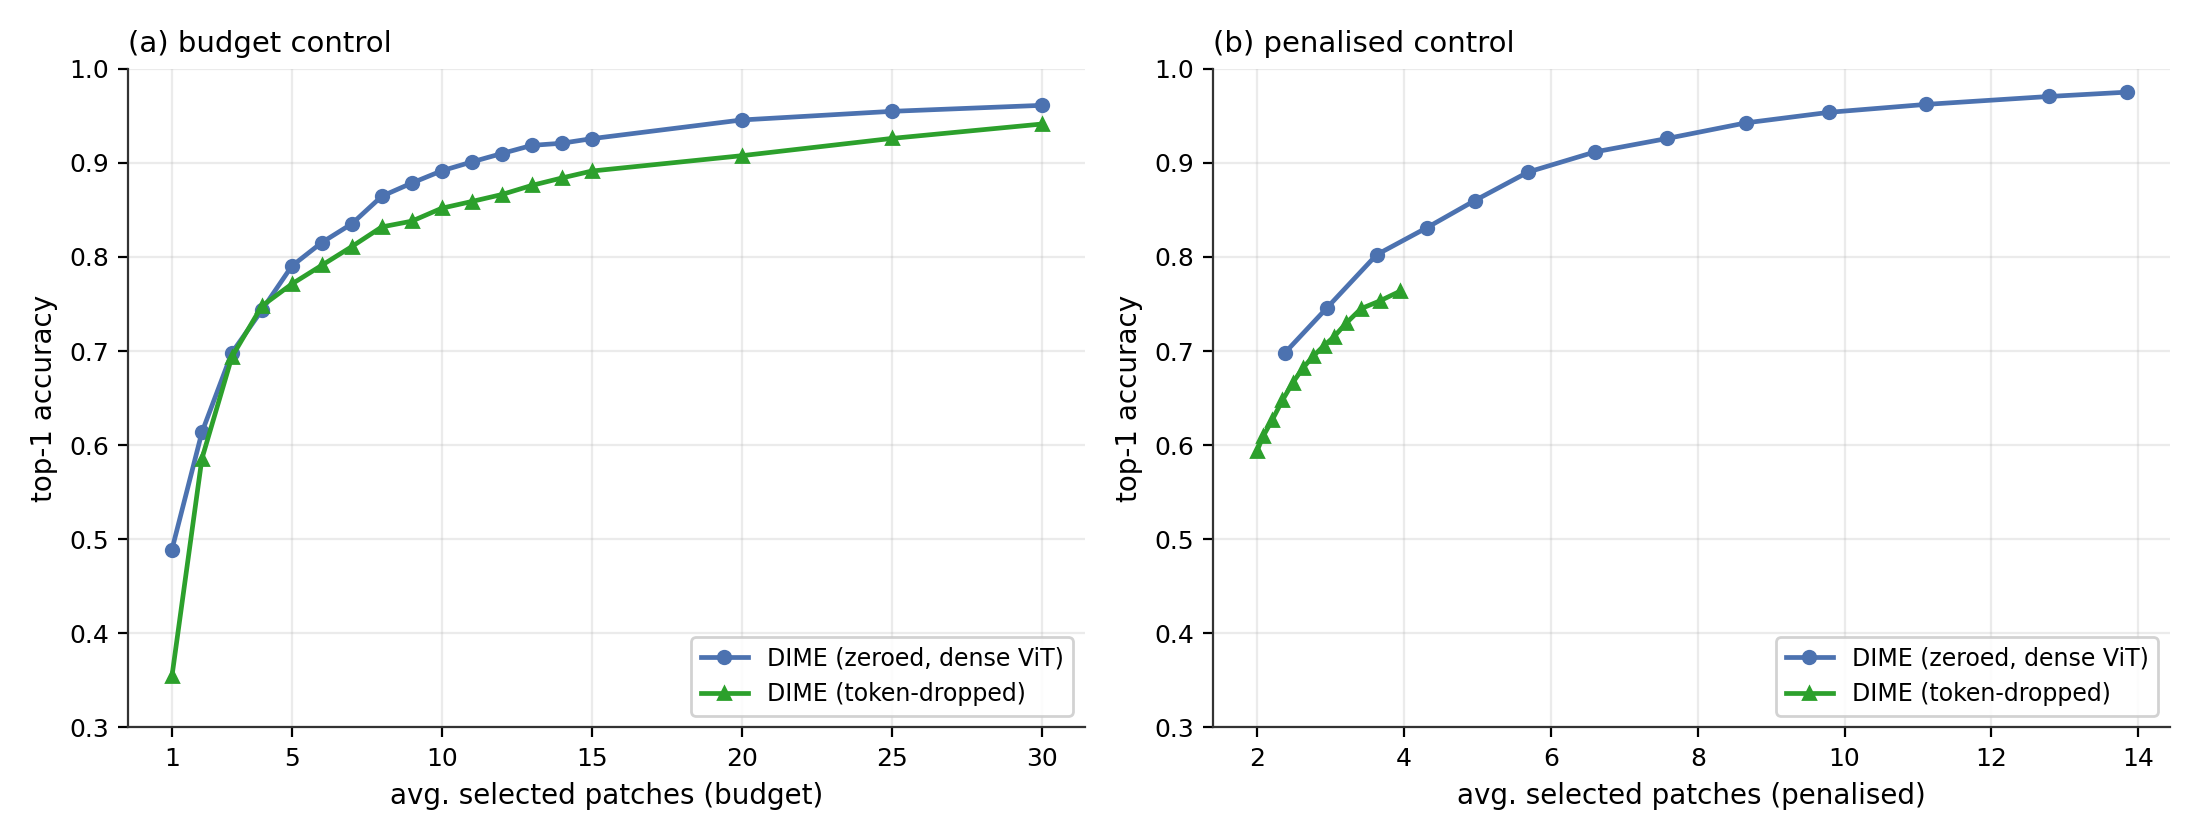
\includegraphics[width=\textwidth]{report_fig10_token_vs_dense.png}
\caption{置零的稠密 ViT 与\tokdrop{} ViT 的准确率曲线。左：预算式；右：惩罚式。}
\label{fig:tokdrop}
\end{figure}

\tokdrop{}版在 5--30 块范围内比置零版低 2--4 个点，1 块时低 13 个点。差距有明确来源：置零版的空 token 带位置编码，等于给单块预测提供了一个学到的空间先验，\tokdrop{}版没有这个先验。它仍高于论文的预算曲线，10 块处高 10 个点。

算力上，它把 $k=10$ 的 FLOPs 倍数从 12$\times$ 压到 0.72$\times$，整个选块过程的算术量比\dense 还少 28\%。读得少，总算得少了。

\subsection{延迟为什么没降}

延迟在空闲 RTX 5060 上重测。训练和精度在 RTX PRO 5000 上完成；测延迟时该卡上还有并行任务，所以下面只比较同一张 5060 上的相对倍数，不跨卡比较绝对毫秒。

但延迟没有跟着降。单图场景（batch 1）下，\tokdrop{}版 $k=10$ 的全程延迟与置零版几乎一样，仍是\dense 的 12 倍。原因在延迟的构成。一次前向的成本可以写成
\begin{equation}
c(n) \approx c_0 + c_1 n,
\end{equation}
$n$ 是 token 数，$c_1$ 是每多一个 token 的边际成本，$c_0$ 是与 token 数无关的\term{固定成本}：读权重、启动 kernel、小矩阵运算的最低开销。eager 下实测一次前向的延迟见表~\ref{tab:fixed} 的 eager 行和图~\ref{fig:fixed}。

\begin{table}[H]
\centering
\caption{丢 token ViT 一次前向的延迟（毫秒，空闲 RTX 5060，eager 执行），随 token 数变化；与图~\ref{fig:fixed} 同一次测量。}
\label{tab:fixed}
\small
\begin{tabular}{lccc}
\toprule
batch & 1 个 token & 16 个 token & 196 个 token \\
\midrule
1 & 7.34 & 7.78 & 7.49 \\
256 & 21.76 & 27.66 & 147.94 \\
\bottomrule
\end{tabular}
\end{table}

\begin{figure}[t]
\centering
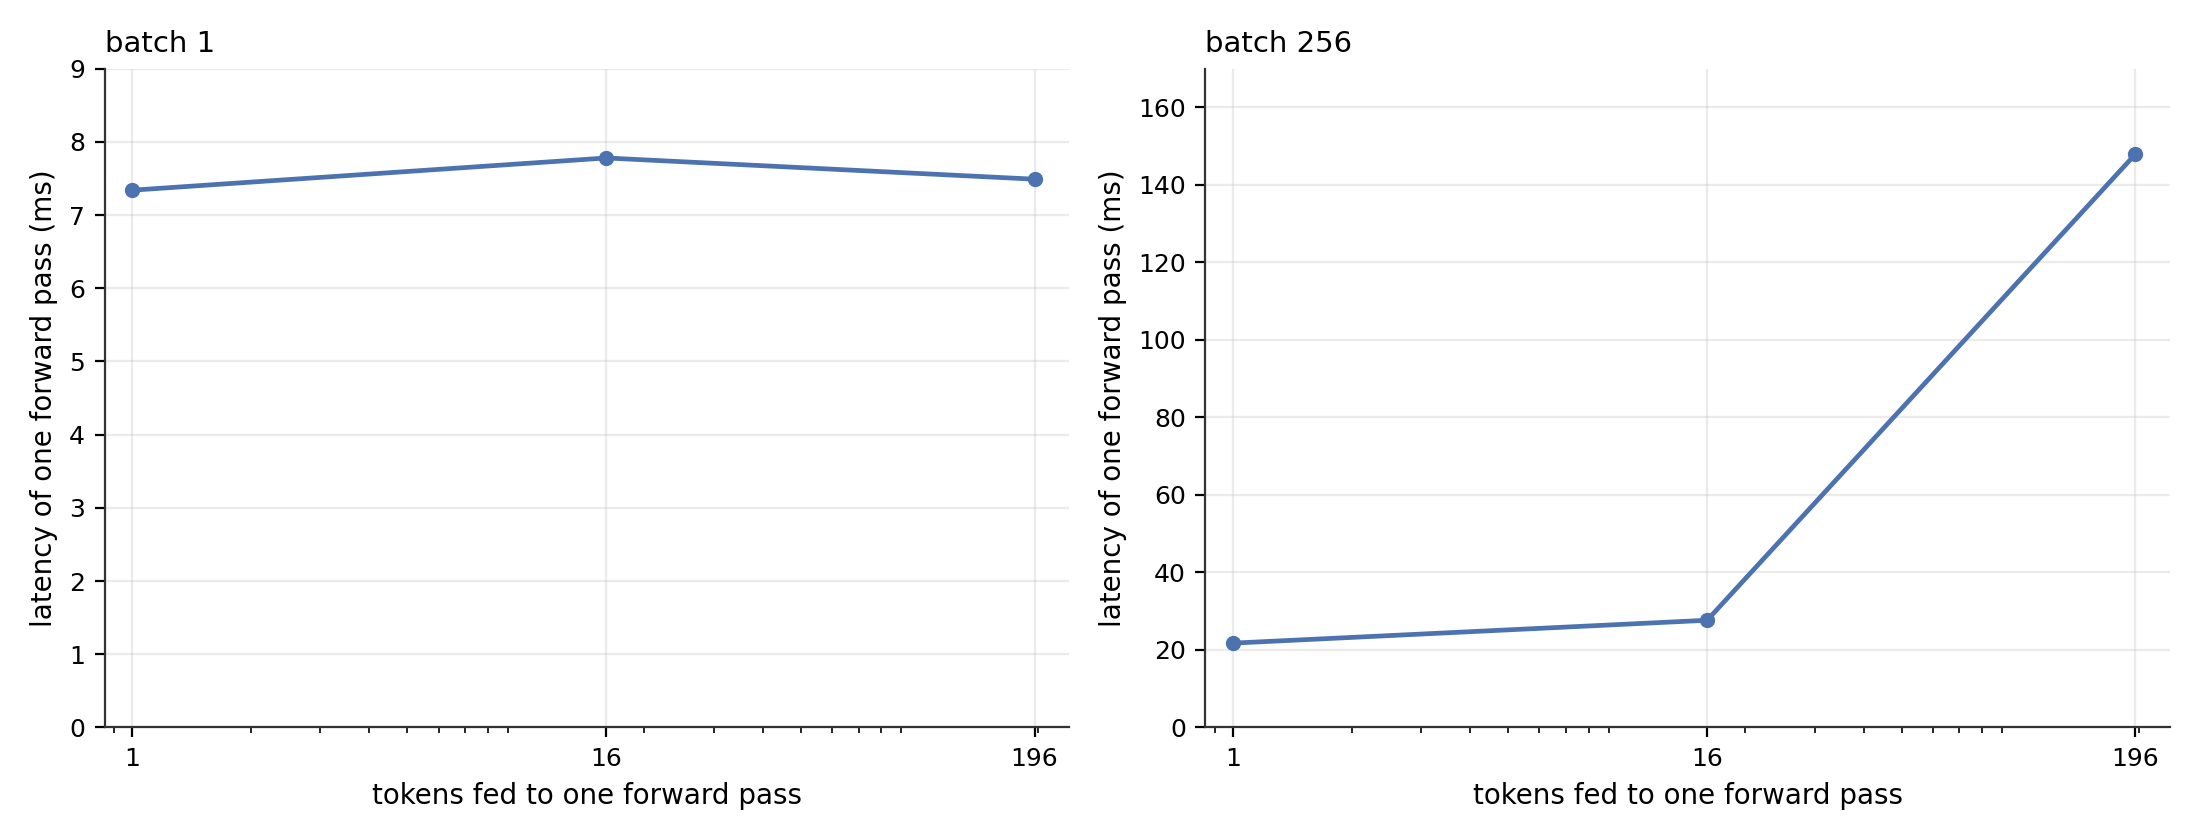
\includegraphics[width=\textwidth]{report_fig06_fixed_cost.png}
\caption{丢 token ViT 一次前向的延迟随 token 数的变化（eager）。batch 1 下几乎与 token 数无关，全是固定成本；batch 256 下固定部分约 22 ms，超出部分才随 token 数增长。}
\label{fig:fixed}
\end{figure}

batch 1 下 1 个和 196 个 token 的前向都在 7.3--7.8 ms，固定成本约 7.3--7.8 ms；batch 256 下固定部分约 22 ms，每多一个 token 约 0.65 ms。也就是说单图场景下\dense 的 7.5 ms 里几乎全是固定成本，少算 185 个 token 省不出时间。预算 $k$ 的推理是 $k+1$ 次前向的串行：
\begin{equation}
C = \sum_{t=0}^{k} c(n_t) + c(n_k),
\end{equation}
每次都要付 $c_0$，次数越多，固定成本叠得越高。这就是为什么\tokdrop{}在单图场景下一点延迟都不省，在吞吐场景（batch 256）下才从 12$\times$ 降到 1.8$\times$。单图场景的延迟瓶颈不是算术量，是“每读一块就串行跑一遍”这个结构本身。

\subsection{压低固定成本}

$c_0$ 本身可以压。torch.compile 的 reduce-overhead 模式用 Triton 把逐元素运算和 LayerNorm 融成少量 kernel，再用 CUDA graph 把整步录成一张图消除启动开销。固定成本从 7.3--21.8 ms 压到 0.73--7.50 ms（表~\ref{tab:fixed-compiled} 与图~\ref{fig:fixed-compiled}）。只把一次前向录成 CUDA graph 而不做算子融合时，$c_0$ 也能降到 0.89--1.30 ms，$k=10$ 的 11 次前向约 10 ms，仍是\dense 的 8 倍；叠加起来 $k=10$ 的全程延迟见表~\ref{tab:stack}。

\begin{table}[H]
\centering
\caption{丢 token ViT 一次前向的延迟（毫秒，空闲 RTX 5060），eager 与 compiled（torch.compile reduce-overhead）对比；eager 行与表~\ref{tab:fixed} 相同，compiled 为同一批测量。}
\label{tab:fixed-compiled}
\small
\begin{tabular}{llccc}
\toprule
batch & 模式 & 1 个 token & 16 个 token & 196 个 token \\
\midrule
1 & eager & 7.34 & 7.78 & 7.49 \\
1 & compiled & 0.81 & 0.73 & 1.19 \\
256 & eager & 21.76 & 27.66 & 147.94 \\
256 & compiled & 7.50 & 13.39 & 112.4 \\
\bottomrule
\end{tabular}
\end{table}

\begin{table}[H]
\centering
\caption{预算 10 块时 DIME 推理的全程延迟（毫秒，空闲 RTX 5060），四层优化逐层叠加，参照是编译后的\dense。}
\label{tab:stack}
\small
\begin{tabular}{lcc}
\toprule
 & batch 1（单图） & batch 256（吞吐） \\
\midrule
作者代码（eager，每步两次前向） & 129.3 & 2757 \\
\fused（eager） & 67.4 & 1438 \\
+ \tokdrop{}（eager） & 82.3 & 260.6 \\
+ 算子融合（compiled） & 8.62 & 103.7 \\
\dense（compiled，参照） & 1.18 & 112.4 \\
\bottomrule
\end{tabular}
\end{table}

表~\ref{tab:stack} 里丢 token 的 eager 行比头融合慢，这是 5060 上的小算子开销：eager 路径每一步都要按已读位置重排 token，价值头还要给 196 个候选位置逐个打分；这些零碎操作摊到 12 次前向上，盖过了省下的矩阵乘。算子融合把这些小算子收拢后，单图才降到 8.6 ms。

\begin{figure}[t]
\centering
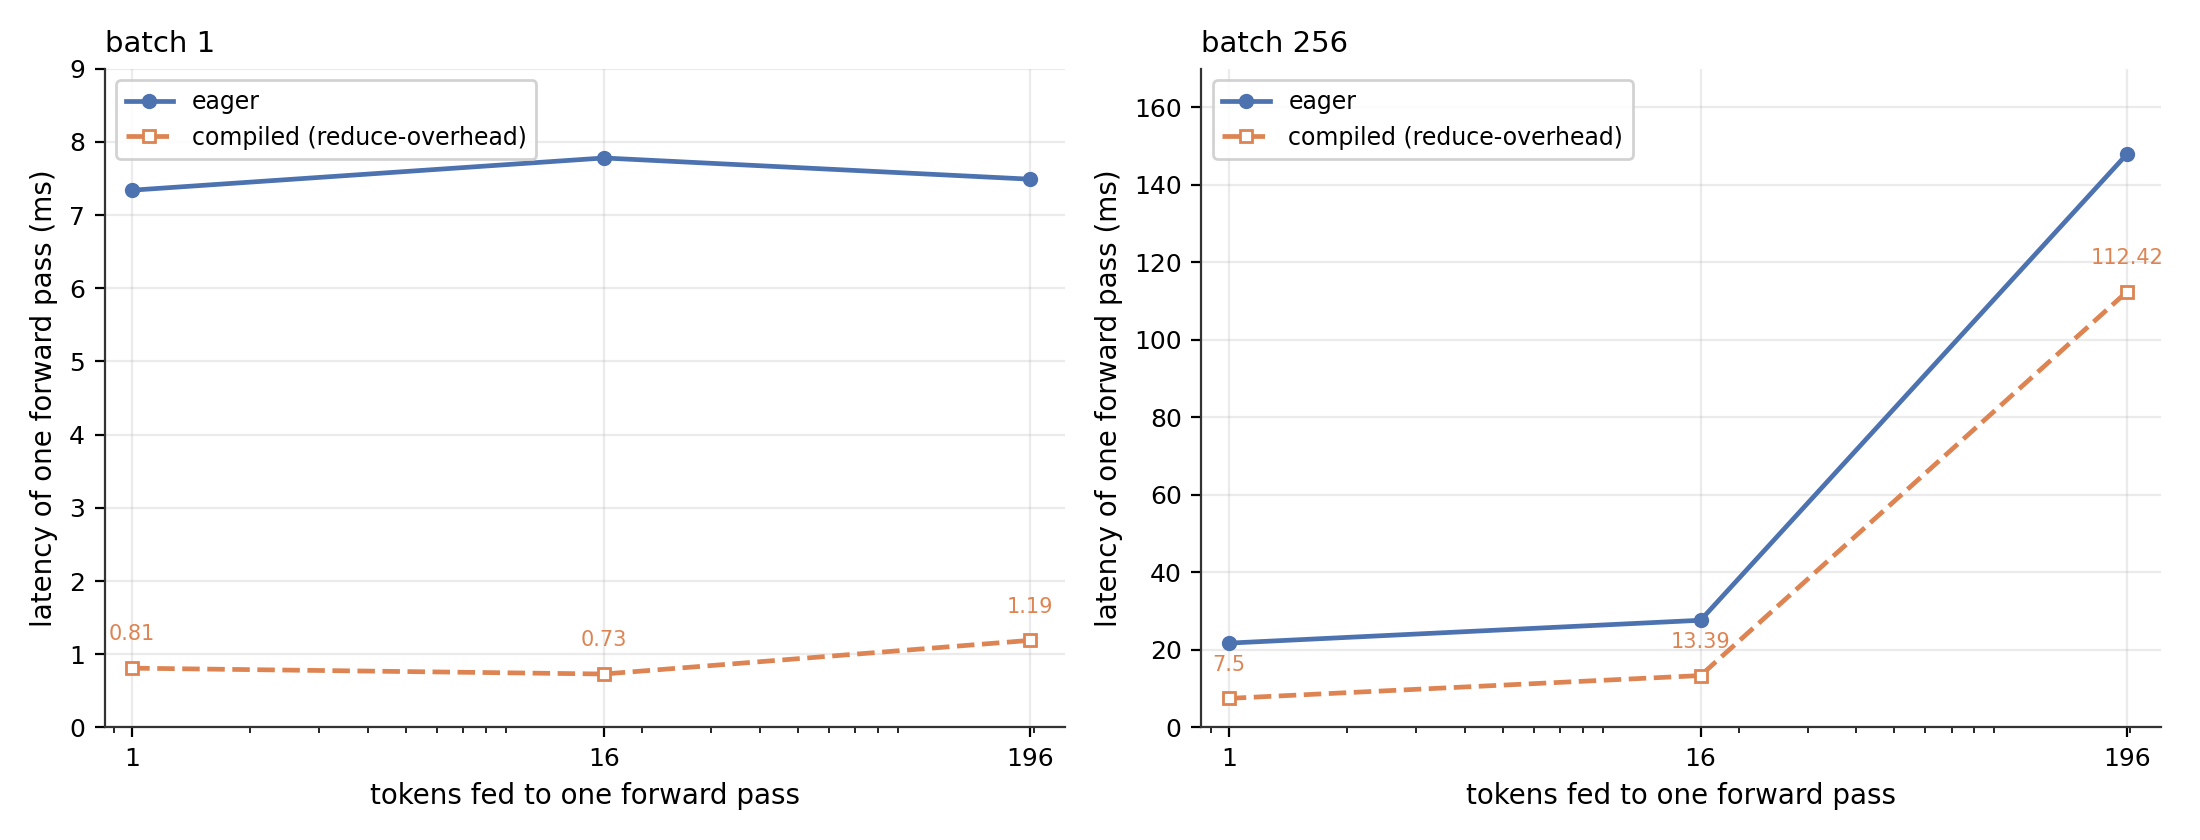
\includegraphics[width=\textwidth]{report_fig06b_fixed_cost_compiled.png}
\caption{算子融合前后，丢 token ViT 一次前向的延迟随 token 数的变化。compiled 把固定成本从 7.3--21.8 ms 压到 0.73--7.50 ms；batch 1 下仍与 token 数几乎无关，batch 256 下 token 数的影响开始占主导。}
\label{fig:fixed-compiled}
\end{figure}

吞吐场景下，\tokdrop{}加算子融合把 $k=10$ 的延迟降到\dense 的 0.92 倍，FLOPs 0.72$\times$，比作者代码快 27 倍：算力和时间同时回到了\dense 的水平。单图场景下从 129 ms 降到 8.6 ms，快 15 倍，但相对\dense 仍是 7.3 倍，因为 11 次串行前向各付 0.81 ms 的固定成本。FLOPs 和吞吐延迟两个目标已经达到，单图场景的延迟受限于结构：固定成本每次 0.81 ms，次数不减，乘积就降不下来。

%----------------------------------------------------------------------------------
\section{第二版改型：把 \texorpdfstring{$k$}{k} 次前向合成一次}
\label{sec:onepass}

\subsection{剩下的杠杆是次数}

延迟等于次数乘每次成本。每次成本已经压到底，次数是唯一剩下的杠杆。最省事的减法是每步多读几块：把每步从读 1 块改成读 $m$ 块，预算 $k$ 的前向次数从 $k+1$ 降到 $\lceil k/m\rceil+1$。用按 $m=1$ 训练好的\tokdrop{}模型直接改推理，不重训，结果见表~\ref{tab:multi}。

\begin{table}[H]
\centering
\caption{每步读 $m$ 块，不重训，只改推理（丢 token 模型，预算式，测试集）。$k=10$ 的前向次数分别为 11 / 6 / 4。}
\label{tab:multi}
\small
\begin{tabular}{lcccccc}
\toprule
块数 & 2 & 4 & 8 & 12 & 16 & 20 \\
\midrule
$m=1$ & 0.585 & 0.748 & 0.832 & 0.866 & & 0.908 \\
$m=2$ & 0.384 & 0.687 & 0.820 & 0.868 & 0.886 & 0.909 \\
$m=4$ & 0.384 & 0.454 & 0.778 & 0.842 & 0.881 & 0.903 \\
\bottomrule
\end{tabular}
\end{table}

每步 2 块在 8 块以上几乎不掉点，前向次数减半；每步 4 块在 8--16 块掉 3--6 点。小预算处掉得多，是因为多块是一起选的：第一步要在什么都没读的情况下选好几块，后面的块只能靠先验，等于浪费。这个实验说明次数可以换，但串行方法的价值恰恰在于“读完一块再推断下一块”，减少次数就是在放弃这个优势。与其一点点放弃，不如把次数降到 1，专门为它设计结构。

\subsection{单趟选块 ViT}

\term{\onepass}把 12 层分成两段。前 $L$ 层叫\term{全图层}（glance layers），照常算 CLS 加全部 196 个 token，与普通 ViT 完全一样。全图层之后\term{选块}一次：第 $L+1$ 层的第一步本来就要算 CLS 对每个 token 的注意力，直接把它当分数，196 个分数取最大的 $k$ 个；其余 $196-k$ 块按注意力加权合成一个\term{汇总 token}，保留一点全局信息。后 $12-L$ 层叫\term{聚焦层}（focus layers），只算 CLS、汇总 token 和 $k$ 个选中块。最后取 CLS 过线性头。

\begin{figure}[t]
\centering
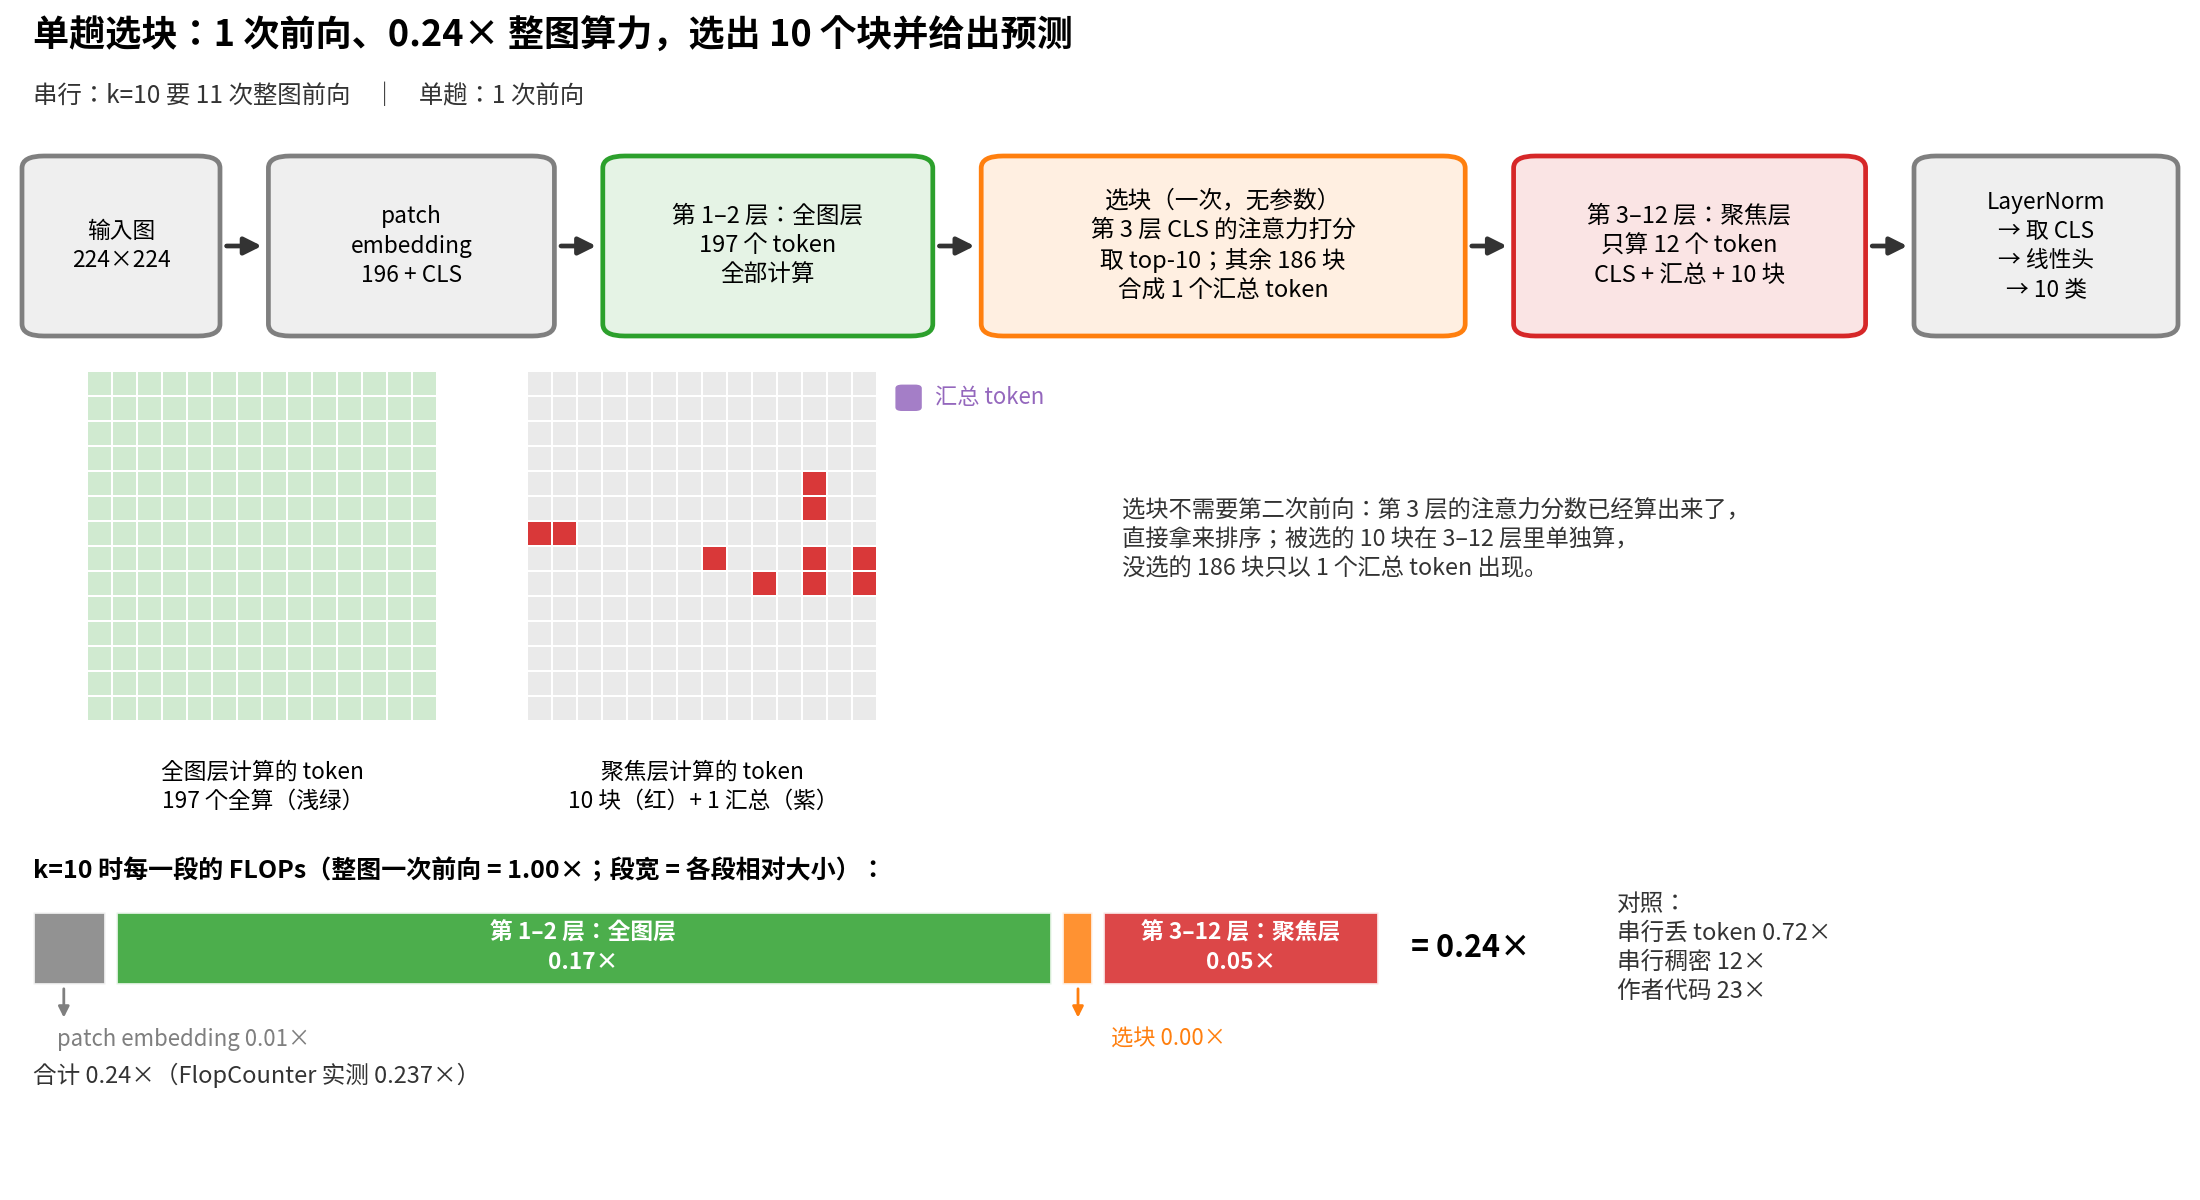
\includegraphics[width=\textwidth]{report_fig09_onepass_arch.png}
\caption{\onepass{}的架构。全图层（前 2 层）算全部 197 个 token；选块用 CLS 的注意力取 top-10，其余 186 块合成 1 个汇总 token；聚焦层（后 10 层）只算 12 个 token。整个过程只有一次前向。}
\label{fig:arch}
\end{figure}

以 $k=10$、$L=2$ 走一遍：$16\times16$ 卷积把图切成 196 个 token，加位置编码，前面拼一个 CLS，共 197 个；第 1、2 层对 197 个 token 做完整的注意力和 MLP；第 3 层里 CLS 的注意力给 196 块打分，取前 10；第 3 到 12 层的输入是 12 个 token；取 CLS 过线性头。整个过程只有一次前向，全图层算完的结果直接被聚焦层接着用，选中的 10 块不重新算，没有“回到输入再跑一遍”的环节。这就是 KV cache 的第二件事，“算过的不重算”，在双向网络里通过只跑一次来实现。

按 FLOPs 实测（\dense 9.4 GFLOPs）：patch embedding 占 0.01$\times$，全图层 2 层占 0.17$\times$，选块可忽略，聚焦层 10 层占 0.05$\times$，合计 0.24$\times$。一般地代价约为
\begin{equation}
\frac{L \cdot 197 + (12 - L)\,(k + 2)}{12 \cdot 197},
\end{equation}
全图层的层数 $L$ 是唯一的旋钮：代价是整图的 $L/12$，$L$ 越大选择越准。

它是串行按需取样的极限：全图层读完后所有块一起选，用“读完一块再推断下一块”换 $k$ 次前向。机制与 EViT（Liang 等，CVPR 2022）相同，本报告把它当作测量工具，不是新机制。

\subsection{训练}

训练要解决两个问题：让单趟模型逼近稠密模型，并让一个模型服务所有预算。损失是标签交叉熵与硬蒸馏各占一半，蒸馏的老师是第 2 节训练好的稠密 DIME 预测器（整图 0.994）：
\begin{equation}
\mathcal{L} = \tfrac12\,\mathrm{CE}(z, y) + \tfrac12\,\mathrm{CE}\big(z,\ \arg\max z^{T}\big).
\end{equation}
$k$ 每个 batch 在 1--30 里随机抽，一个模型服务所有预算。AdamW，学习率 $10^{-5}$ 余弦衰减，batch 32，最多 60 轮，验证集取 $k=5/10/20$ 的平均准确率做早停。数据、骨干、增强与串行实验相同。训练里没有 rollout，单卡单任务 8 秒一轮，每个运行 0.12--0.2 GPU 小时，比串行训练便宜两个数量级。

\subsection{准确率}

\begin{table}[H]
\centering
\caption{\onepass{}在 Imagenette 测试集上的准确率（种子 0），随全图层层数 $L$ 与预算 $k$ 变化。最后一列是 $k=10$ 时的 FLOPs，相对\dense；$L=3$ 和 6 为按 token 数推算。最后两行是串行 DIME 的两种版本。}
\label{tab:onepass-acc}
\footnotesize
\setlength{\tabcolsep}{5pt}
\begin{tabular}{lccccccc}
\toprule
$L$ & $k=2$ & 5 & 10 & 15 & 20 & 30 & FLOPs@$k=10$ \\
\midrule
1 & 0.770 & 0.842 & 0.899 & 0.926 & 0.945 & 0.965 & 0.203$\times$ \\
2 & 0.839 & 0.875 & 0.917 & 0.931 & 0.947 & 0.967 & 0.237$\times$ \\
3 & 0.893 & 0.918 & 0.937 & 0.956 & 0.963 & 0.971 & 约 0.31$\times$ \\
4 & 0.909 & 0.931 & 0.949 & 0.960 & 0.970 & 0.977 & 0.389$\times$ \\
6 & 0.936 & 0.952 & 0.965 & 0.974 & 0.979 & 0.983 & 约 0.55$\times$ \\
\midrule
串行 DIME（置零） & 0.614 & 0.790 & 0.892 & 0.926 & 0.946 & 0.961 & 12$\times$ \\
串行 DIME（\tokdrop） & 0.586 & 0.771 & 0.852 & 0.891 & 0.908 & 0.941 & 0.72$\times$ \\
\bottomrule
\end{tabular}
\end{table}

\begin{table}[H]
\centering
\caption{\onepass{}的三种子结果（均值 $\pm$ 样本标准差）。}
\label{tab:seeds}
\footnotesize
\setlength{\tabcolsep}{4pt}
\begin{tabular}{lcccccc}
\toprule
配置 & $k=2$ & 5 & 10 & 15 & 20 & 30 \\
\midrule
全图层 $L=2$ & 0.840$\pm$0.003 & 0.876$\pm$0.003 & 0.915$\pm$0.002 & 0.936$\pm$0.005 & 0.950$\pm$0.002 & 0.966$\pm$0.001 \\
全图层 $L=4$ & 0.911$\pm$0.002 & 0.932$\pm$0.002 & 0.951$\pm$0.001 & 0.962$\pm$0.003 & 0.970$\pm$0.001 & 0.978$\pm$0.002 \\
\bottomrule
\end{tabular}
\end{table}

\begin{figure}[t]
\centering
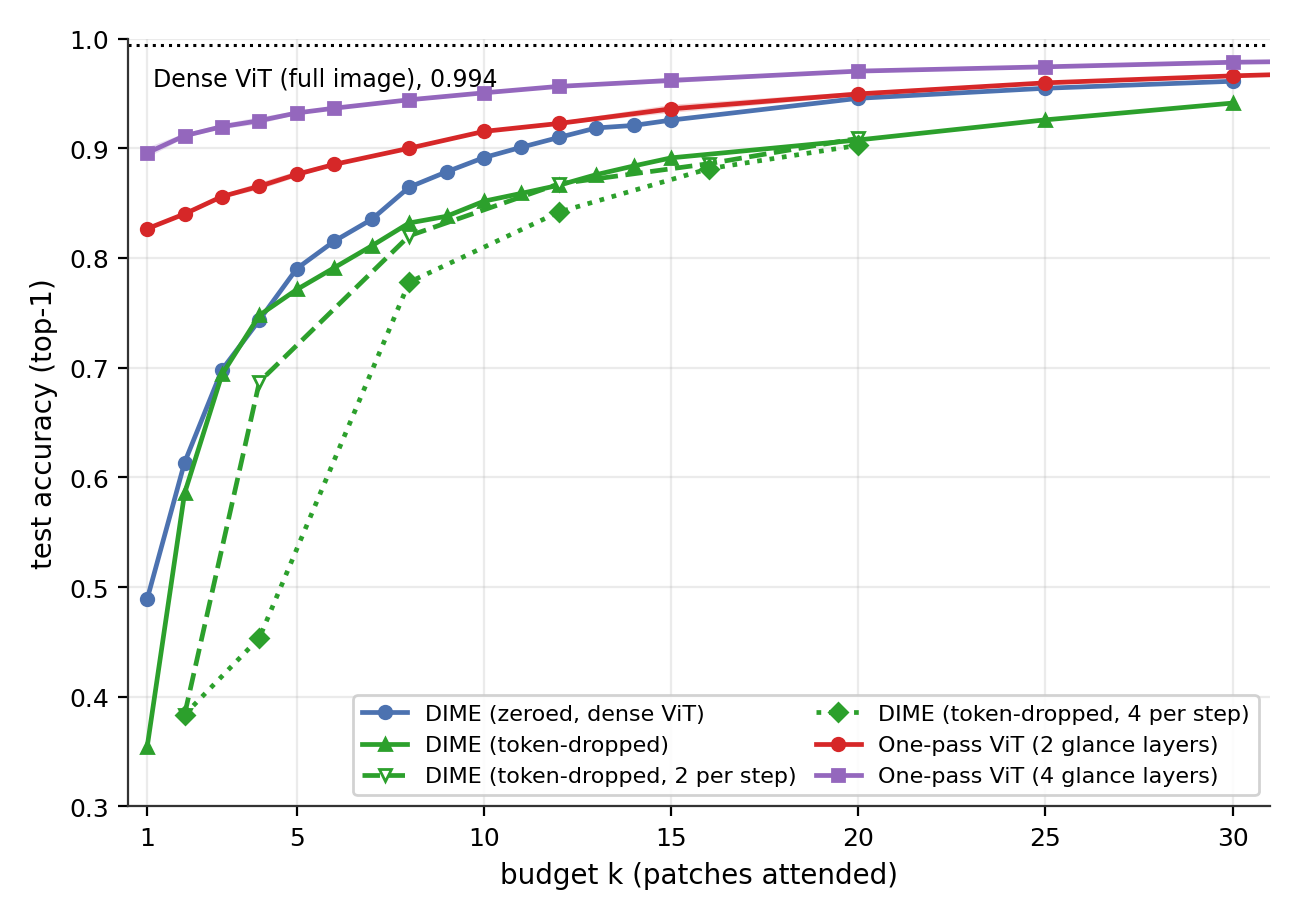
\includegraphics[width=0.8\textwidth]{report_fig11_accuracy_budget.png}
\caption{准确率随预算的变化：串行按需取样（蓝、绿）与\onepass{}（红、紫，三种子均值 $\pm$ 标准差）。}
\label{fig:acc-budget}
\end{figure}

表~\ref{tab:onepass-acc} 是种子 0 的准确率随 $L$ 与 $k$ 的变化，表~\ref{tab:seeds} 是三种子的均值与标准差。同一预算下单趟更准：$k=10$ 时 $L=2$ 比串行置零版高 2.3 个点、比串行\tokdrop{}版高 6.3 个点；$L=4$ 与串行最好的惩罚式（9.8 块 0.954）持平，$L=6$ 超过它。原因是全图层读了全部 196 块，这是串行方法在 $k=10$ 时做不到的。种子间差异在 0.5 个点以内。$L$ 从 1 增到 4，小预算处准确率上升最快，到 6 饱和。

两项消融（$L=2$）：固定 $k=10$ 训练 0.914，随机 $k$ 0.917，一个模型服务所有预算不掉点；去掉蒸馏 0.900，蒸馏值 1.7 个点。满预算（196 块）时 $L=2$ 为 0.992，与\dense 的 0.994 相当；$L=4$ 为 0.980，因为聚焦层从未见过全部 token，满预算时直接用稠密模型即可。

\subsection{算力与延迟}

\begin{table}[H]
\centering
\caption{预算 10 块时的算力与延迟（Imagenette，空闲 RTX 5060，bf16）。compiled 指 torch.compile reduce-overhead 模式；\dense 一行是同一模型 $k=196$ 的路径，与单趟模型同一会话同一张卡测得。}
\label{tab:onepass-cost}
\small
\begin{tabular}{lccccc}
\toprule
方法 & 前向次数 & FLOPs & batch 1 & batch 256 & 准确率 \\
\midrule
作者代码（eager） & 23 & 23$\times$ & 129 ms & 2757 ms & \\
\fused{}（eager） & 12 & 12$\times$ & 67.4 ms & 1438 ms & 0.892 \\
\tokdrop{}（eager） & 11 & 0.72$\times$ & 82.3 ms & 261 ms & 0.852 \\
\tokdrop{}（compiled） & 11 & 0.72$\times$ & 8.62 ms & 104 ms & 0.852 \\
\onepass{} $L=2$（eager） & 1 & 0.24$\times$ & 6.58 ms & 35.7 ms & 0.917 \\
\onepass{} $L=2$（compiled） & 1 & 0.24$\times$ & 0.87 ms & 29.6 ms & 0.917 \\
\onepass{} $L=4$（compiled） & 1 & 0.39$\times$ & 1.01 ms & 43.0 ms & 0.949 \\
\dense（compiled，参照） & 1 & 1$\times$ & 1.18 ms & 100.6 ms & 0.994 \\
\bottomrule
\end{tabular}
\end{table}

\begin{figure}[t]
\centering
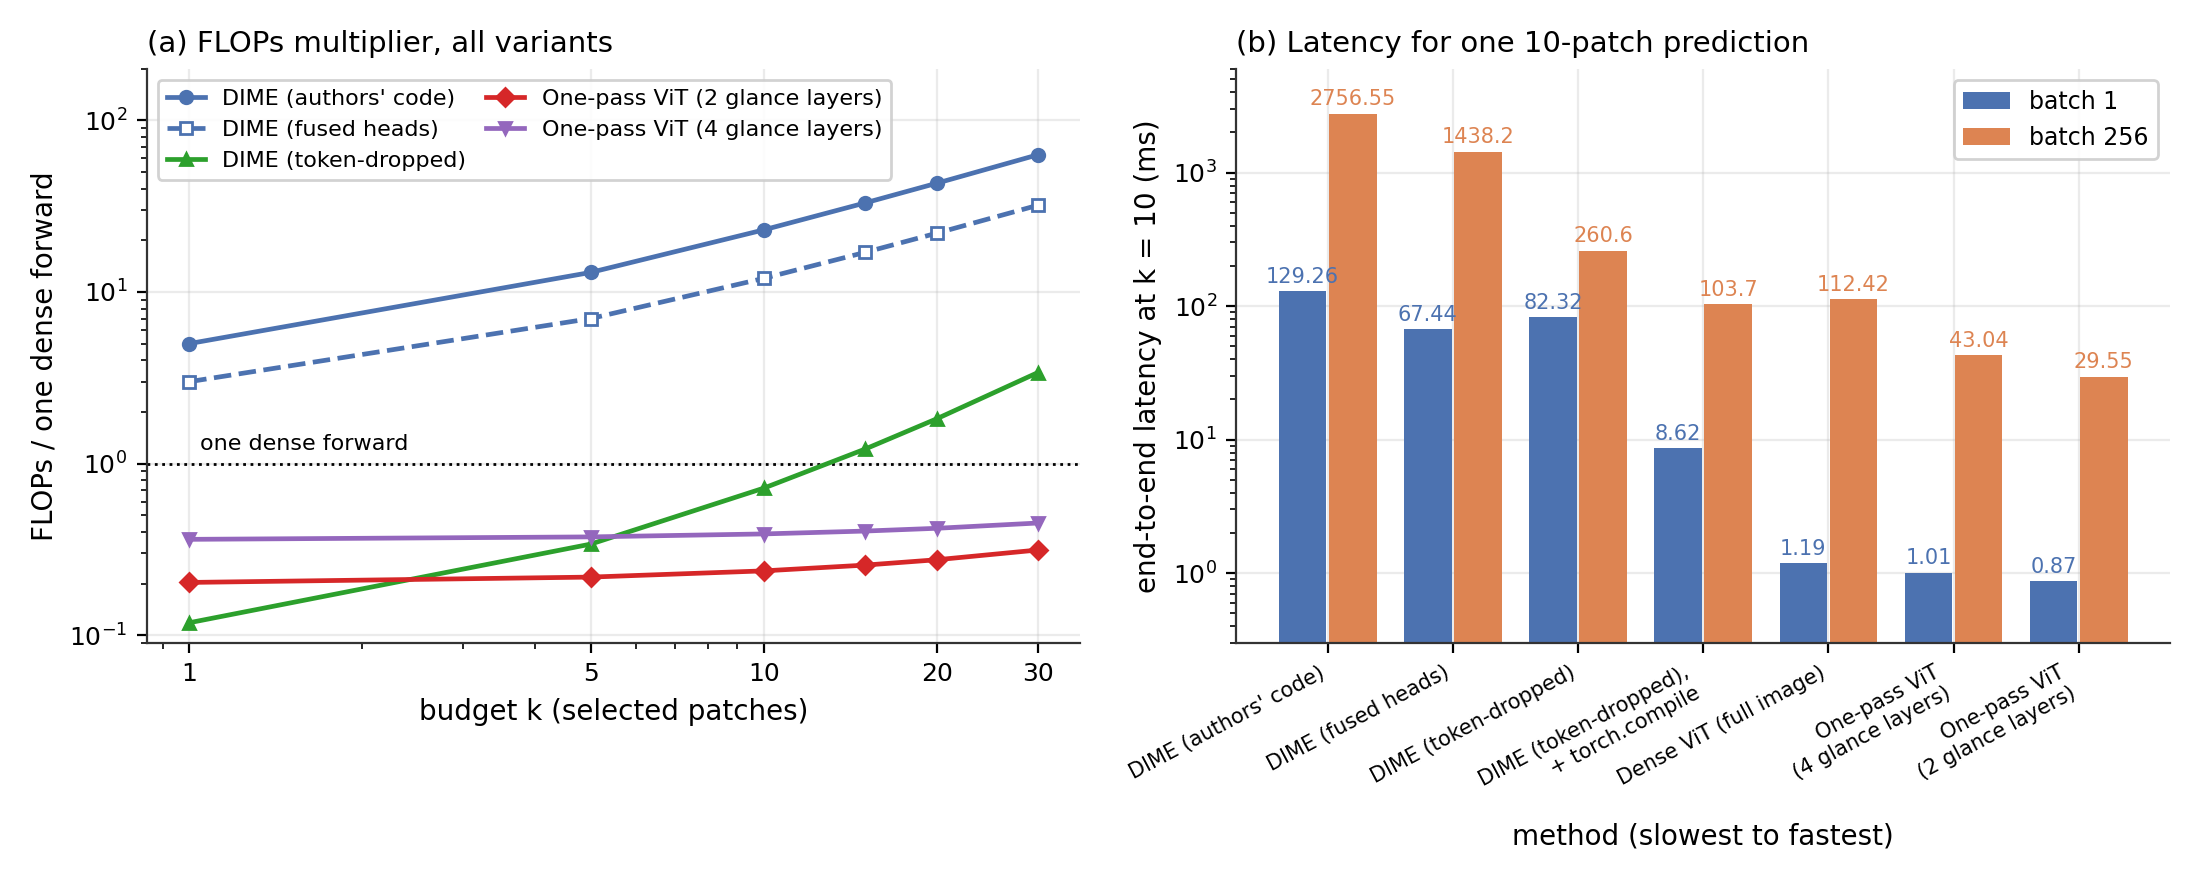
\includegraphics[width=\textwidth]{report_fig14_ledger_full.png}
\caption{所有改型的算力与延迟对比（Imagenette，预算 $k$）。左：FLOPs 相对\dense 的倍数随预算的变化。右：预算 10 块时的全程延迟，batch 1 与 batch 256；\tokdrop{}、\onepass{}和参照为 compiled 测量，作者代码与\fused{}为 eager 测量。}
\label{fig:ledger-full}
\end{figure}

\begin{figure}[H]
\centering
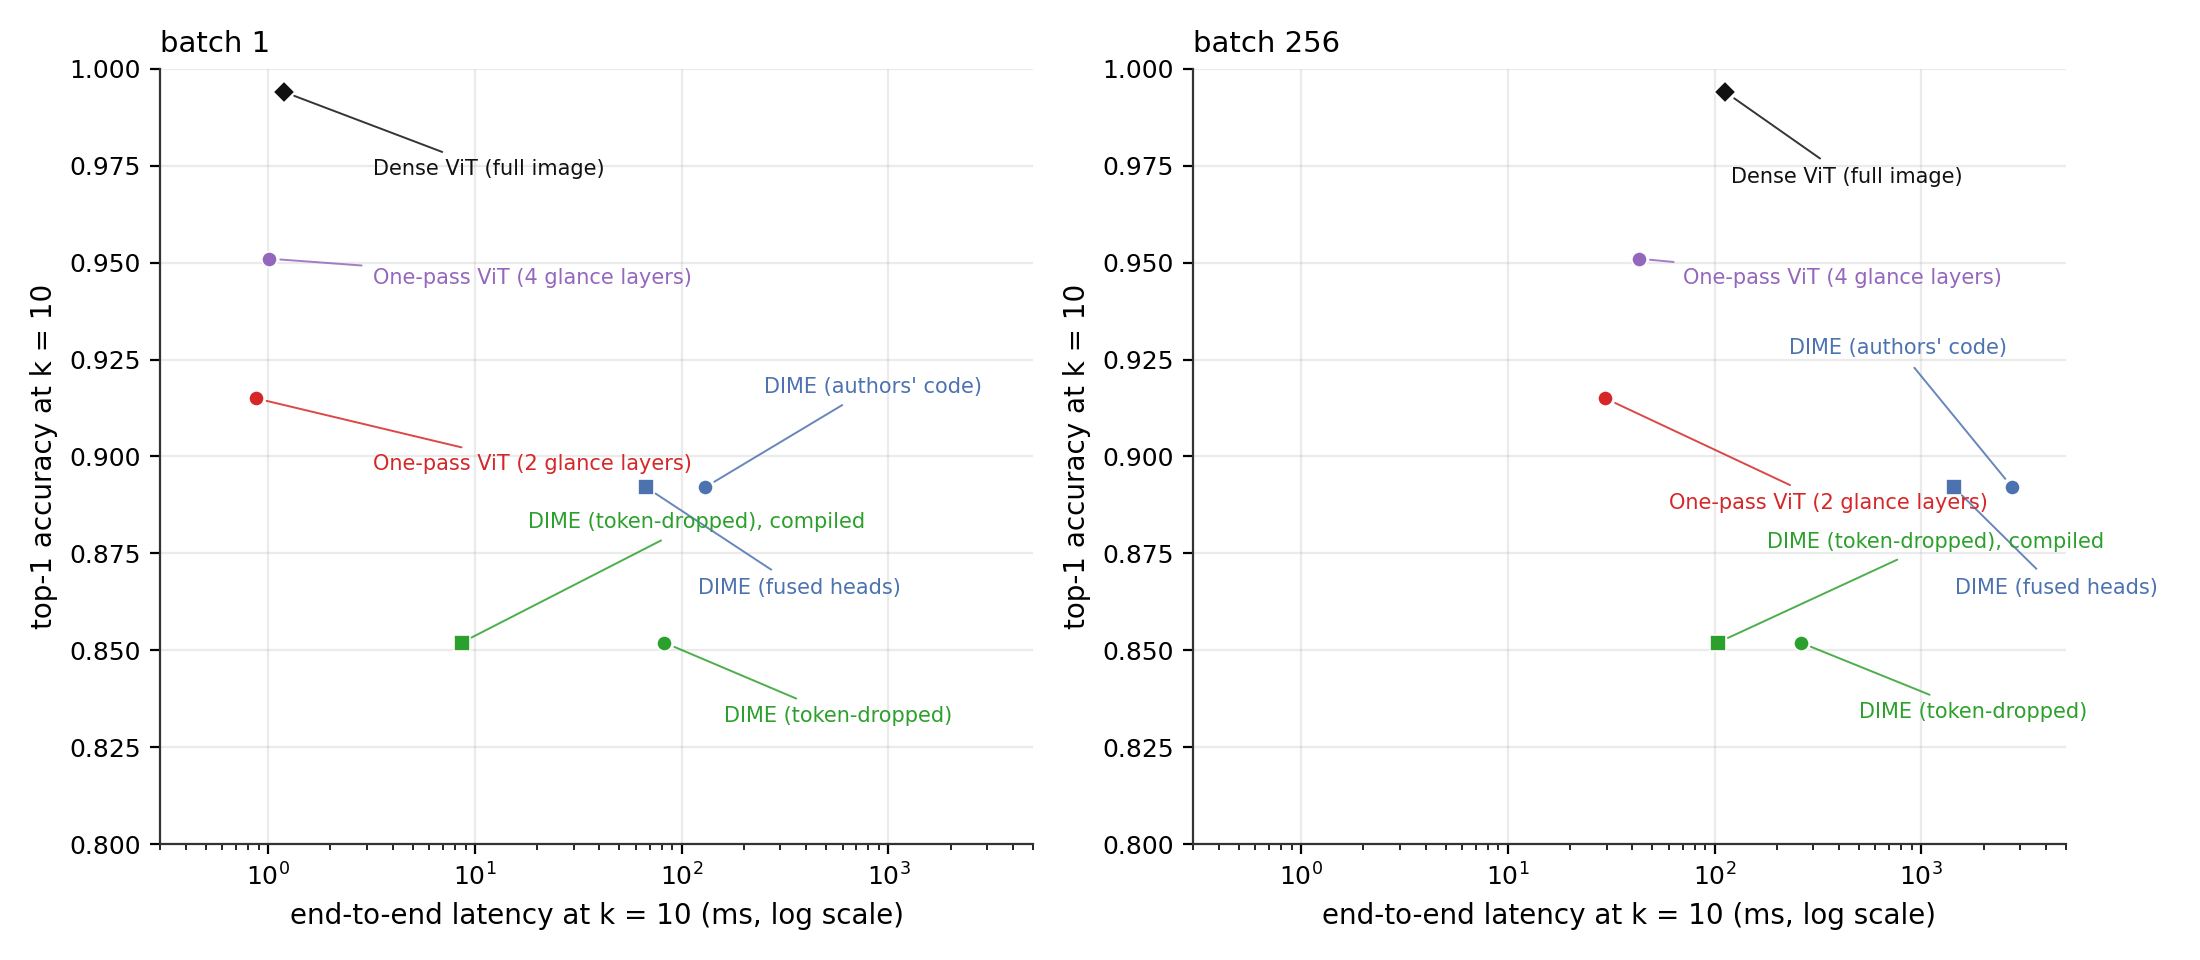
\includegraphics[width=\textwidth]{report_fig12_pareto.png}
\caption{预算 10 块时的延迟与准确率，每个方法一个点。左：单图场景（batch 1）；右：吞吐场景（batch 256）。}
\label{fig:pareto}
\end{figure}

算力上，$k=10$ 时 FLOPs 只有 0.24$\times$\dense，相当于串行\tokdrop{}的三分之一、作者代码的 1/97。

延迟在吞吐场景下是\dense 的 0.29 倍，比串行\tokdrop{}快 3.5 倍，比作者代码快 93 倍：这是 FLOPs 节省转化为时间的场景，吞吐场景下边际成本 $c_1 n$ 占九成。延迟在单图场景下是\dense 的 0.74 倍，只省 26\%。回到第 4.3 节的那条平线：单图场景下 12 层里每层约 98 微秒的固定成本与 token 数无关，\dense 的 1.18 ms 本来就是这个地板，少算 token 省不出时间。\onepass{}在单图场景下的收益被这个地板限制，但仍比串行 compiled 快 9.9 倍。如果单图延迟是硬需求，剩下的杠杆只有减层数或减宽度，那是另一个问题。

\subsection{读了哪些块}

\begin{figure}[t]
\centering
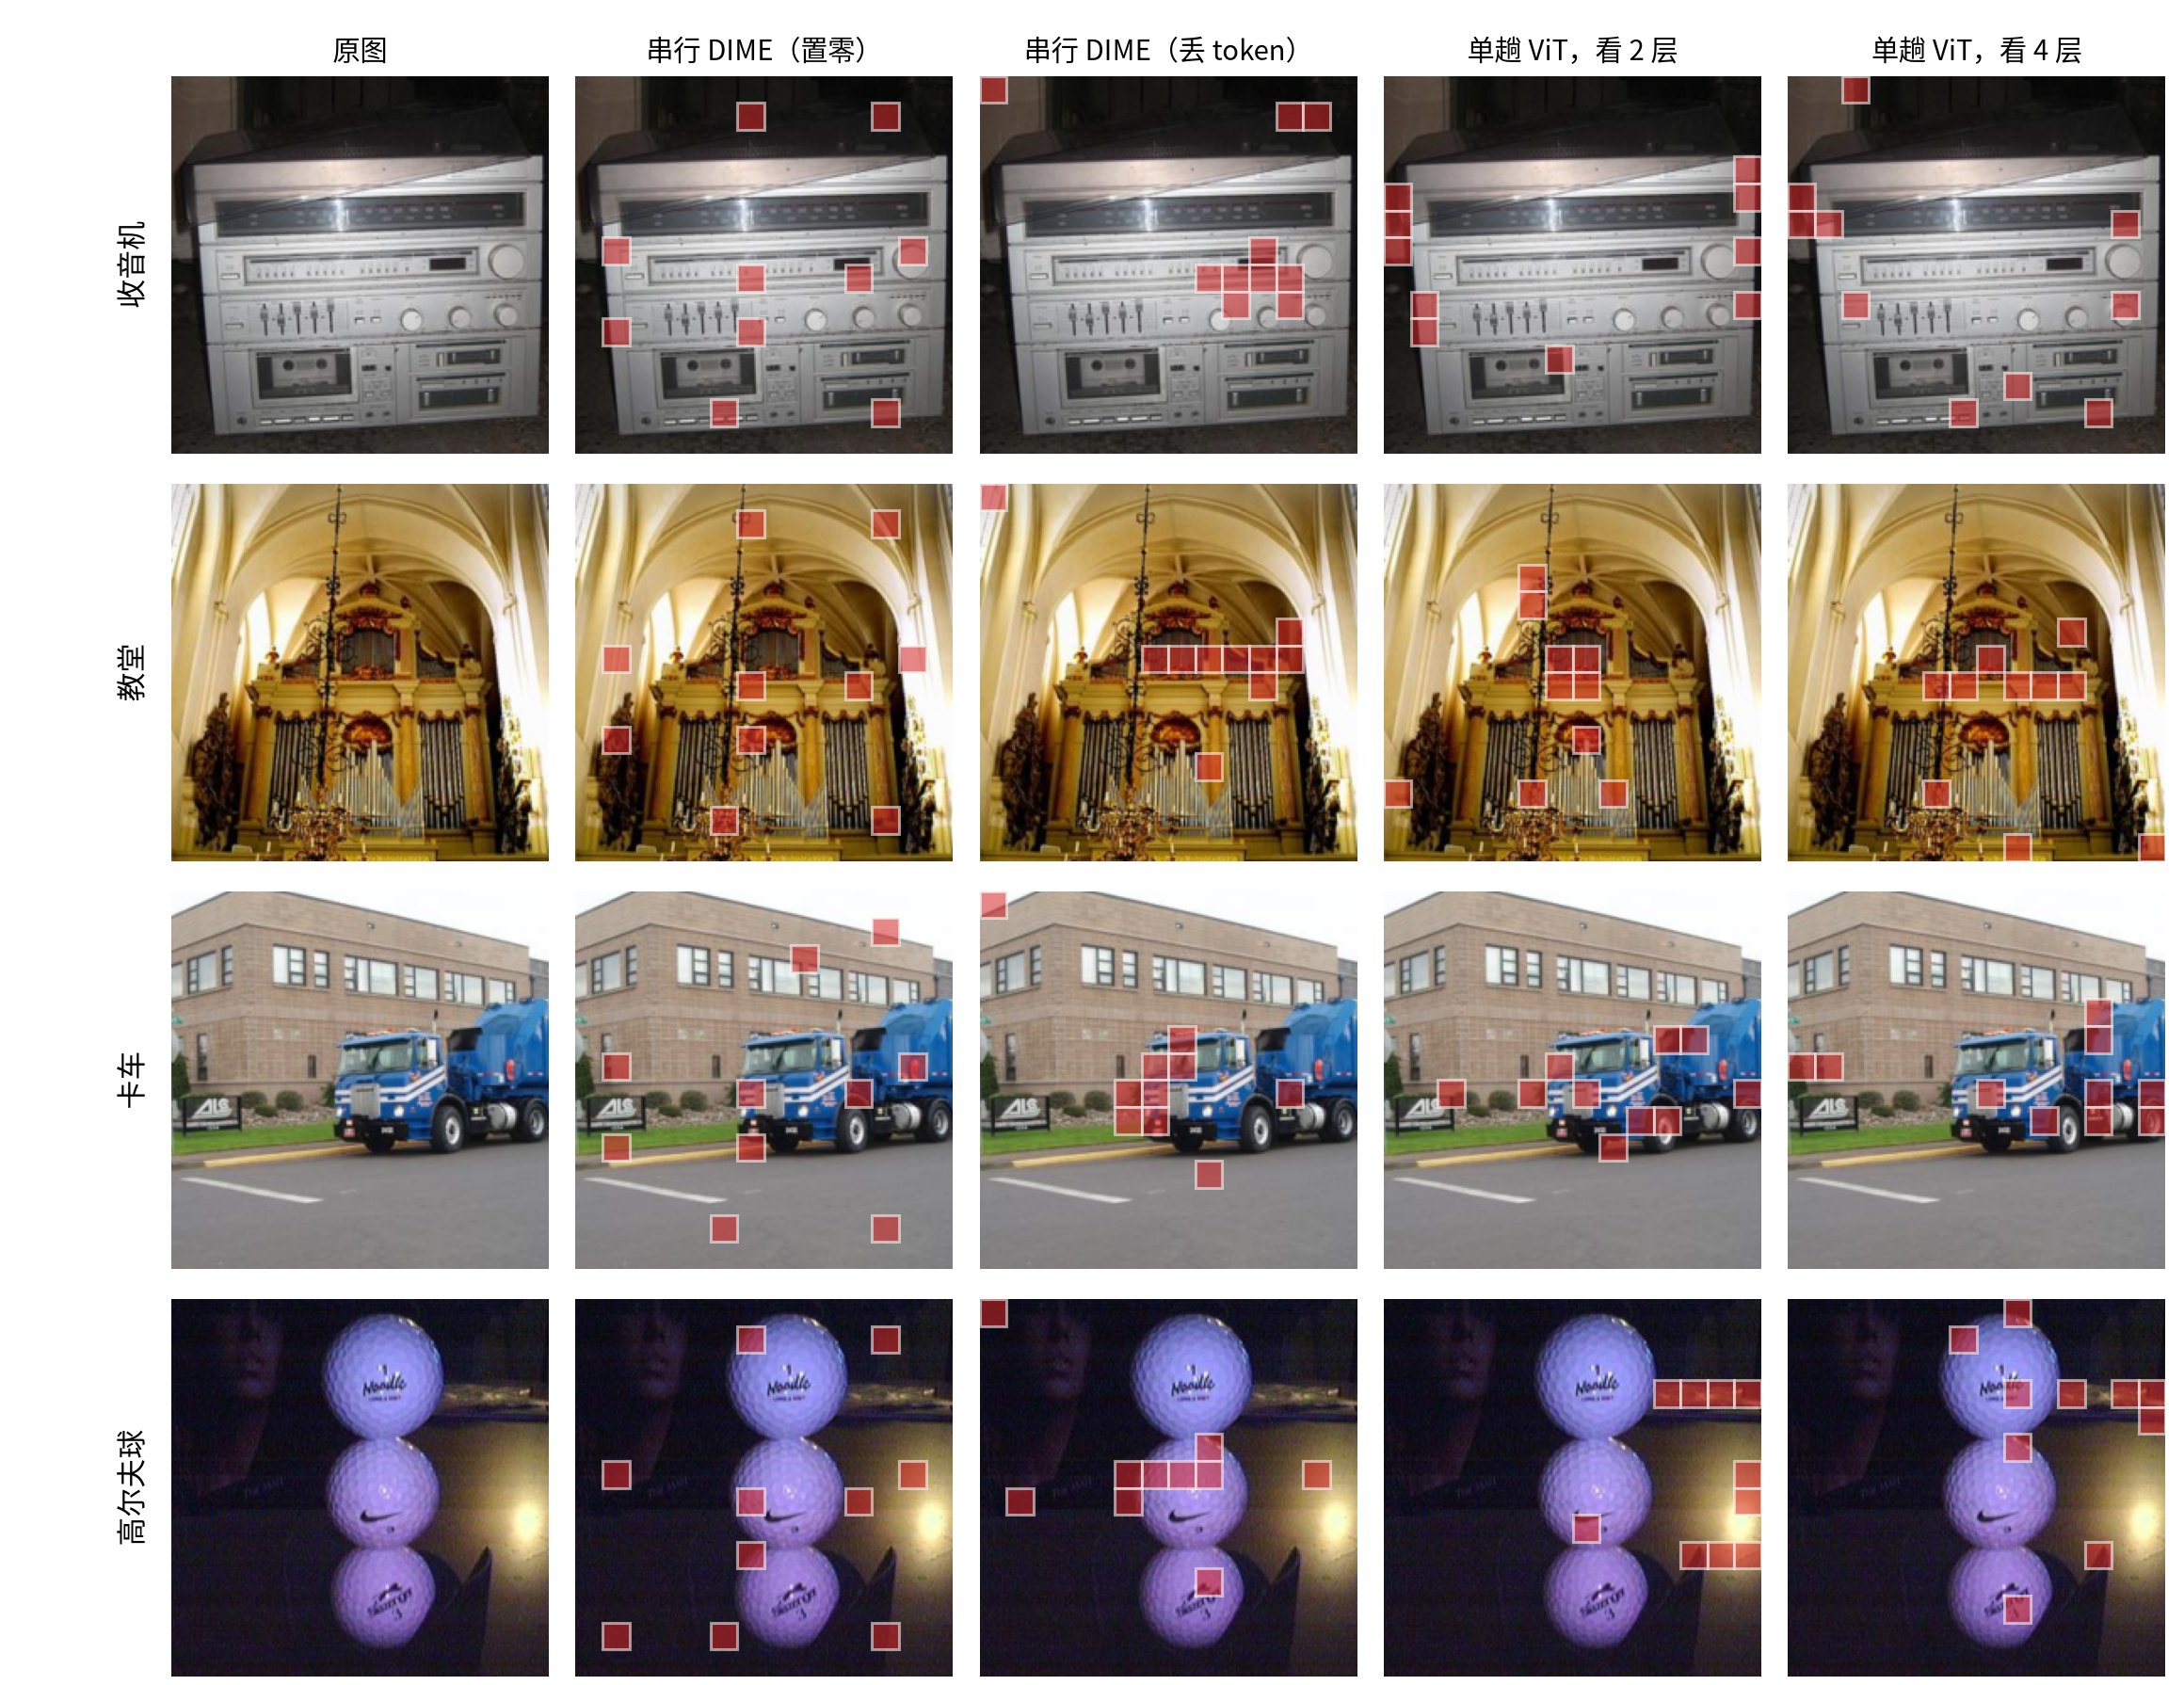
\includegraphics[width=\textwidth]{report_fig13_selected_patches.png}
\caption{预算 10 块时各方法读入的块（红色），Imagenette 测试集。}
\label{fig:qualitative}
\end{figure}

串行置零版选得散，常选到四角和背景，与第 4.2 节的观察一致：置零版的空 token 带位置编码，模型学会了用位置先验补信息。串行\tokdrop{}版选得集中，落在物体上。\onepass{}两种都落在物体上，$L=4$ 比 $L=2$ 更集中在判别性区域（收音机的旋钮和磁带仓、卡车的驾驶室、高尔夫球）。这是定性观察，只检查了四张图，没有量化。

\subsection{代价}

\onepass{}用一次前向换掉了“读完一块再推断下一块”。它的全图层读了全图，所以它和串行方法在“只读 $k$ 块”的意义上不是同一个任务，只在算力和延迟的意义上才是公平比较。这个区别不是措辞问题，它对应两个真实场景。

在获取成本场景里，串行按需取样是对的。每读一块都有真实成本，比如医疗影像的剂量、传感器采样、传输带宽、隐私；串行方法真的只获取了 $k$ 块，延迟和算力不是目标。第 3 节的算力对比在这个场景下不是批评，只是代价说明。

在算力场景里，评价标准换成同准确率下的计算量。像素免费，“只读 $k$ 块”没有独立价值，全图粗读再聚焦 $k$ 块是更合理的设计，串行结构比它贵一个数量级。第 5.5 节的比较在这个场景下成立。

%----------------------------------------------------------------------------------
\section{讨论}

\subsection{结论}

\begin{enumerate}
\item 复现成立。GDFS 在 MNIST 和 CIFAR-10、DIME 在 MNIST 和 Imagenette 上的曲线达到或高于论文，验收线全部通过；“少量特征能保持精度”这个前提成立。
\item 算力悖论成立，来源是结构。按作者代码，预算 10 块时 GDFS 是\dense 的 14 倍 FLOPs，DIME 是 23 倍；未读的块置零后照样经过每一层。稀疏卷积在 CNN 上的上界只有 7\%，ViT 上可以把未读的块从计算里删掉。
\item 删掉未读的块能省 FLOPs，省不了单图延迟。\tokdrop{} ViT 把 FLOPs 压到 0.72$\times$，一次前向的固定成本压到 0.81 ms 之后，单图延迟仍是\dense 的 7.3 倍，因为延迟等于前向次数乘每次前向的固定成本，串行结构的前向次数是 $k+1$。
\item 把前向次数降到 1 之后，算力和延迟同时下降。\onepass{}在 $k=10$ 时 FLOPs 0.24$\times$，吞吐场景延迟 0.29$\times$，单图场景延迟 0.74$\times$，准确率 0.915，反而比串行方法高 2--6 个点。
\item 单图场景的延迟地板与 token 数无关。\onepass{}在单图场景只省 26\%，因为 12 层每层约 98 微秒的固定成本构成了\dense 的 1.18 ms。单图场景下再往下只能减层或减宽。
\item 两个场景要分开。串行按需取样适合获取成本场景；算力场景应该用单趟结构，并按“同准确率”而不是“同预算”比较。
\end{enumerate}

\subsection{局限}

算力实验只在一个数据集上做（Imagenette），CNN 上只有上界计算没有实现，所以“稀疏卷积不划算”这个判断在 CNN 上是上界证据，不是实测。复现主结果是单种子；\onepass{}给了三种子，种子差异 0.5 个点以内。串行\tokdrop{}版比置零版低 2--4 个点，没有达到“不超过 3 个点”的线。\onepass{}的满预算路径准确率略低于稠密（$L=2$ 时 0.992 对 0.994），满预算时应直接用稠密模型。定性图只检查了四张。编译后的数值与 eager 的 logit 偏差在 L=2 时约 0.01--0.2，L=4、k=10 的个别路径可达 1.8；精度评测仍用 eager。

\subsection{相关工作}

单趟选块的机制不是新的。DynamicViT（Rao 等，ICLR 2021）用可学习的预测模块按比例逐步丢 token 并用蒸馏；EViT（Liang 等，CVPR 2022）用 CLS 注意力打分并把丢掉的 token 融合成一个；A-ViT（Estrada 等，CVPR 2022）让每个 token 自适应决定在哪一层停止；GFNet（Wang 等，NeurIPS 2021）先低分辨率读一遍，再在高分辨率上细读。本报告的贡献不在机制，而在把动态特征选择的两篇工作与这条线接起来：同一模型、同一数据、同一张卡上，把串行、每步多块、单趟三种结构的前向次数和每次前向成本分解测出来。

%----------------------------------------------------------------------------------
\section{LLM 领域实验}

本节预留给并行进行的 LLM 领域实验。并入时按同样的框架写：问题、方法原理、设置、结果、算力与延迟账本、与本文结论的对应。

%----------------------------------------------------------------------------------
\appendix
\section{实现细节与与作者设定的偏离}
\label{app:dev}

\begin{table}[H]
\centering
\caption{与作者设定的偏离。}
\footnotesize
\setlength{\tabcolsep}{4pt}
\begin{tabular}{>{\raggedright\arraybackslash}p{2.4cm}>{\raggedright\arraybackslash}p{2.5cm}>{\raggedright\arraybackslash}p{2.4cm}>{\raggedright\arraybackslash}p{4.4cm}>{\raggedright\arraybackslash}p{2.9cm}}
\toprule
项目 & 作者 & 我们 & 原因 & 影响 \\
\midrule
框架 & PyTorch Lightning 1.x & 纯 PyTorch 逐行移植 & Lightning 1.x 与 Blackwell 需要的 torch $\geq$ 2.7 不兼容 & 语义相同 \\
CIFAR 选择头输出 & 代码 $16\times16$，论文 $8\times8$ & $8\times8$ & 作者代码与 $8\times8$ 掩码不匹配，无法运行 & 按论文 \\
混合精度 & fp16 & bf16 & 新硬件更稳 & 数值级差异 \\
DIME ViT 前向 & 两个头各跑一次骨干 & 合成一次前向 & 两头共享骨干，结果逐元素相同 & 训练快一倍，结果相同 \\
DIME MNIST checkpoint & 监控准确率但 mode=min & mode=max & 作者脚本 bug & 避免选到最差轮次 \\
DIME 预训练权重 & 保留最后一轮 & 同作者 & 照搬 & 同作者 \\
MNIST 训练步 & eager & 整步 CUDA graph & 多任务共卡时快 10 倍以上 & 单步逐参数一致（误差 $7\times10^{-9}$） \\
评测 & 每个预算重新选一遍 & 一次选到最大预算并逐步记录 & 选择是确定性 argmax & 结果相同 \\
\bottomrule
\end{tabular}
\end{table}

单趟选块的实现：\path{src/patchdfs/sparse/onepass.py}；训练与评测：\path{onepass_train.py}（支持 \texttt{-{}-eval-only}）；配置 \path{configs/sparse/imagenette_onepass.yaml}；启动脚本 \path{scripts/run_onepass.sh}。丢 token ViT：\path{src/patchdfs/sparse/token_vit.py}。单元测试 28 项通过，其中一项验证 $k=196$ 且不合并汇总 token 时\onepass{}与稠密 ViT 逐 logit 一致。

\section{复现状态表}

\begin{table}[H]
\centering
\caption{实验状态与验收。}
\small
\small
\begin{tabular}{>{\raggedright\arraybackslash}p{4.8cm}>{\raggedright\arraybackslash}p{1.3cm}>{\raggedright\arraybackslash}p{8.6cm}}
\toprule
实验 & 状态 & 验收 \\
\midrule
GDFS MNIST & 完成 & 过 \\
GDFS CIFAR-10 & 完成 & 过 \\
DIME MNIST & 完成 & 过 \\
DIME Imagenette 稠密 & 完成 & 过 \\
基线：中心裁剪、随机掩码、CAE & 完成 & 趋势一致 \\
算力账本 & 完成 & \\
稀疏卷积上界 & 完成 & 不写核 \\
\tokdrop{}版 & 完成 & 准确率差 3--4 点，未达 $\leq$ 3 点；延迟见第 4 节 \\
算子融合 & 完成 & \\
每步多块 & 完成 & \\
\onepass{} & 完成 & $k=10$ 三种子 $L=2$ 0.915、$L=4$ 0.951；FLOPs 0.24/0.39$\times$；吞吐延迟 0.29/0.43$\times$；单图延迟 0.74/0.86$\times$ \\
\bottomrule
\end{tabular}
\end{table}

\section{文件索引}

\begin{table}[H]
\centering
\small
\setlength{\tabcolsep}{4pt}
\begin{tabular}{>{\raggedright\arraybackslash}p{3.2cm}>{\raggedright\arraybackslash}p{12.0cm}}
\toprule
内容 & 位置 \\
\midrule
全部数字（权威） & \path{docs/RESULTS.md} \\
复现步骤 & \path{docs/REPRODUCE.md} \\
GDFS 复现 & \path{src/patchdfs/gdfs/}，\path{configs/gdfs/}，\path{scripts/run_gdfs.sh} \\
DIME 复现与推理 & \path{src/patchdfs/dime/}，\path{configs/dime/}，\path{scripts/run_dime.sh} \\
丢 token ViT & \path{src/patchdfs/sparse/token_vit.py}，\path{configs/sparse/imagenette_token.yaml} \\
\onepass{} & \path{src/patchdfs/sparse/onepass.py}，\path{onepass_train.py}，\path{configs/sparse/imagenette_onepass.yaml} \\
稀疏卷积上界 & \path{src/patchdfs/sparse/conv_bound.py} \\
算力账本 & \path{src/patchdfs/bench/}，\path{results/compute_ledger/} \\
延迟与 FLOPs 脚本 & \path{scripts/figures/lat_compile_vit.py}，\path{lat_onepass.py} \\
报告图 & \path{results/report_fig*.png}，生成脚本 \path{scripts/figures/report_figs_data.py}，\path{report_figs_concept.py} \\
作者代码只读副本 & \path{third_party/dynamic-selection}，\path{third_party/DIME} \\
\bottomrule
\end{tabular}
\end{table}

\end{document}
